% $Id: ESMF_archdoc.tex,v 1.6 2002/08/19 23:16:19 cdeluca Exp $

%
\documentclass[]{article}

\usepackage[dvips]{graphics,color}
\usepackage{epsf}
\usepackage{html}
\usepackage[T1]{fontenc}

\textwidth 6.5in
\textheight 8.5in
\addtolength{\oddsidemargin}{-.75in}

\begin{document}

\bodytext{BGCOLOR=white LINK=#083194 VLINK=#21004A}

\begin{titlepage}

\begin{center}
{\Large Earth System Modeling Framework } \\
\vspace{.25in}
{\Large {\bf ESMF Architecture}} \\
\vspace{.25in}
{\large {\it DRAFT}}
\vspace{.5in}
\end{center}

\begin{latexonly}
\vspace{5.5in}
\begin{tabular}{p{5in}p{.9in}}
\hrulefill \\
\noindent {\bf NASA High Performance Computing and Communications Program} \\
\noindent Earth and Space Sciences Project \\
\noindent CAN 00-OES-01 \\
\noindent http://www.esmf.ucar.edu \\
\end{tabular}
\end{latexonly}

\end{titlepage}

\tableofcontents

\newpage
%section{Synopsis}
%\section{Synopsis}

The following document describes the general scope and requirements
of the initial Earth System Modeling Framework.









\newpage
\begin{htmlonly}
\addcontentsline{toc}{part}{Overview}
\end{htmlonly}
\part{Overview}
\label{part:Overview}

%\section{Introduction}

{\it 
In this section, we describe: 
\begin{itemize}
\item the goals and unique role of ESMF in Earth science;
\item the relevant features of the problem domain that ESMF encompasses; and
\item the key design features that are derived from the requirements of the ESMF domain and 
enable the ESMF to satisfy its goals. 
\end{itemize}
}

The {\bf Earth System Modeling Framework (ESMF)} is a software toolkit that increases 
software reuse, component interoperability, performance portability, and ease of use in 
Earth science applications.  The focus on Earth systems - a diverse but bounded domain - is 
critical to the ability of the ESMF to achieve its goals.  This is where the ESMF's value and 
capability come from - enabling interoperability but able to retain some efficiency and structure 
because the domain is bounded.  The scope is also unique - there are larger projects and smaller 
projects, but only ESMF spans institutions that are all interested in collaboration. The fifteen 
initial testbeds for the ESMF represent a wide range of research and operational applications in 
climate, weather, and data assimilation \cite{ref:models}.  Thus the ESMF must efficiently 
support a variety of grids, programming paradigms, and computing platforms.  However, the ESMF 
domain is restricted enough to allow the creation of specific data and control constructs.  A 
challenge of the project is to support high-performance operations in the face of the generality 
that's required.  Commonality in applications can be found at both the {\bf infrastructure} 
level, in model development tools for communication, I/O, time management, and other basic 
functions; and at the {\b superstructure} level, in an architecture and standards for 
combining geophysical components into applications.

The ESMF design is rooted in the requirements and characteristics of the applications that 
the framework must support.  In the sections below, these characteristics are described.  
Then we describe the major architectural implications that spring from the nature of the 
domain.

The key characteristics of the Earth science code that the ESMF must address are as follows.
\begin{enumerate}

\item Applications contain sets of complex software components that represent different 
physical domains, such as land, ocean, atmosphere and sea ice.  Other components may perform 
data assimilation or analysis.  These components are "coupled" so that the output fields of 
some of the components are used 
as the input fields for other components.  Coupling may include data transfers, unit 
conversions, flux 
calculations, regridding, data transfers, and other transformations.  The software that 
couples components is often viewed as a component itself.  

\item The same models or components may be run in a variety of configurations.  Scientists 
may swap in
alternative implementations of a domain or function in order to create new applications 
(e.g., different 
ocean models, different dynamical cores); may use different subsets and combinations 
of a particular set of 
components (e.g., an atmospheric model may be run with an ocean model for a 
hurricane application, and 
with a full complement of land, ocean, and sea ice models for a climate simulation); may 
run ensembles of the same component; and as a matter of course attempt endless variations 
and combinations of these research strategies.

\item Applications run on a variety of parallel computing systems and require high performances. 

\item Applications have many diverse users, from graduate students to software engineers 
to .  Applications are under continuous scientific development, and scientists and developers 
frequently wish to modify and update the code.

\end{enumerate}

The characteristics above inform a software architecture.  The key architectural features 
of ESMF are described below.

\begin{description}
\item[Component-based architecture]  Applications running under ESMF are organized as sets of 
interacting {\bf Components}.  A Component is
a software representation of some domain or function; for example, a land model or data 
assimilation 
system.  All Components share common behavior in ESMF.  This architectural model lends itself 
naturally to systems whose functionality is segregable.

\item[Types of Components]  ESMF Components fall into a number of categories.  The two primary 
types are Gridded 
Components ({\tt ESMF\_GridComp}) and ESMF Coupler Components ({\tt ESMF\_CplComp}).  A 
Gridded Component represents 
a physical domain that contains fields discretized on a grid.  A Coupler Component performs the operations required for two or more components to interact with each other.

\item[Local communication]

One of the important features of the ESMF architecture is that all communication between 
Gridded Components is 
local.  Another way of stating this is that all inter-component communication is mediated 
by a Coupler Component.    
\end{description}























%\section{Scope}
\section{Scope of the ESMF}
\label{sec:shortscope}

The ESMF includes
\begin{itemize}
\item services and standards for coupling high-level model components; and 
\item an infrastructure of general utilities for composing model components.
\end{itemize}  
The model components we will support initially are those included in the ESMF {\it Joint 
Milestone Codeset (JMC)}, which consists of fifteen climate, weather and data 
assimilation applications.
These codes, developed by ESMF investigators and their colleagues, include the National 
Centers for Environmental Prediction (NCEP) Forecast 
Suite \cite{parrish, derber1}, applications running under the Geophysical Fluid Dynamics
Laboratory (GFDL) Flexible Modeling System (FMS) \cite{fms}, applications running under 
the Goddard Earth Modeling System {GEMS} \cite{gems}, the Community Climate System 
Model (CCSM) \cite{ccsm}, the Weather Research and Forecast Model (WRF) \cite{wrf}, and 
more.  A full listing of JMC codes is available on the ESMF website, 
\htmladdnormallink{http://www.esmf.ucar.edu}{http://www.esmf.ucar.edu},
via the {\bf Applications} link on the navigation bar.  

Components of the JMC applications include regional and global atmospheres, regional and 
global oceans, land models, sea ice models, and data assimilation systems.  Components will 
recode or wrap their internal data structures in order to provide a standard ESMF interface 
and employ ESMF intercomponent communications.  The ESMF coupling services will include 
software for representing data distributions, interpolating and redistributing gridded data, 
and load balancing computations.

Coupling services will be built upon a base of general data structures and utilities.
Data structures and associated methods are defined for common constructs such as 
fields and grids.  
Supporting the coupling services and accessible to model developers are a set of 
general ESMF utilities.  These include error handling, timing and profiling, 
message logging, low-level I/O and communication, time management, and parameter 
specification.

\begin{figure}
\begin{center}
\scalebox{0.7}{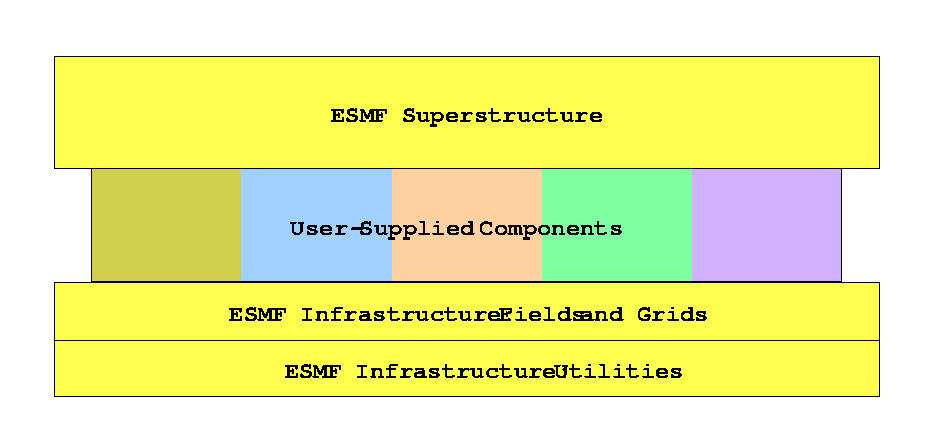
\includegraphics{Sandwich.eps}}
\caption[{ESMF Architecture}] {The simplest view of the ESMF architecture
is that it consists of an infrastructure for developing components and 
a superstructure for assembling applications.}
\label{fig:sandwich}
\end{center}
\end{figure}









%\section{Terminology}
\section{Terminology}

The computers on which large Earth system models run are complex, multi-part
systems that vary considerably in structure, as are Earth system applications 
themselves.  Thus as we begin the task of composing a modular software
infrastructure that incorporates constructs from both computer hardware 
and physical systems, we find that there are a multitude of ways to impose 
categories and layers.  In this section we define a set of terms -- some standard,
some not -- describing alternative ways of deconstructing Earth system applications
and the ESMF.  These terms will help to clarify subsequent discussions.

\subsection{Object-Oriented Design}

The ESMF will be designed using object-oriented (OO) principles.  OO design
is characterized by the use of {\it classes}, and the related strategies of
{\it encapsulation}, {\it inheritance}, and {\it polymorphism}.  Classes 
organize data, attributes, and associated methods into well-defined structures.
Encapsulation means making class data inaccessible so that the underlying representation
can be changed or extended without changing the user interface to the class.
Inheritance allows specialized classes to inherit basic behaviors from generic
classes.  Polymorphism allows a single method to be overloaded for use 
when performing conceptually similar operations.  Together these OO
strategies help to organize and streamline codes, making them more flexible,
maintainable, and extensible.

\subsection{Modes of Parallelism}

We use the term {\bf data parallel} to describe an operation performed
on data that is distributed over multiple memory locations and that typically
represents portions of a single physical quantity.  Roughly the same
calculation occurs on all processors at the same time.  Most individual 
model components are run in a data-parallel fashion.

By {\bf task parallel} we mean operations performed on multiple data sets 
distributed over non-overlapping sets of memory locations.  Typically 
each data 
set represents a different physical system, and the calculations performed
on each set are different as well.

\subsection{Sequencing}

Sequential execution of model components describes the case in which 
one component waits for the other to finish before it begins
to execute.  Components may be in the same or different executables
and may have identical or non-overlapping memory distributions.

Concurrent execution of model components occurs when two components,
whether in the same or different executables, execute simultaneously.

\subsection{Layering Methodologies}

Layering generally refers to a calling hierarchy, in which upper layers 
call lower layers.  While this explains how layers {\it work}, it doesn't 
explain what a layer {\it is}.  In this section we describe some common 
layering approaches.  

We use the term {\bf hardware layering} to refer to a strategy to encapsulate 
programming constructs and tools that reflect the structure of the underlying 
computing environment.  In hardware layering, a bottom layer typically includes 
vendor-specific constructs.  A representative higher layer may automatically 
handle standard operations, such as distributed transposes, that are not  
vendor-specific but still reflect architectural details.  At the application layer 
the user handles objects that represent the application 
domain and not the computing environment.  

Hardware layering is one form of {\bf layering by generality}; general 
tools that can apply to many domains are relegated to bottom layers, 
while domain-specific constructs are in top layers.  This paradigm is
common even in systems running on simpler hardware architectures, where vendor-specific
constructs and other threats to portability and ease of use are not a concern.
Its pervasiveness is simply a reflection of the fact that general tools 
enable a variety of applications to be built upon them.

An alternative view of layers results from combining multiple modes of parallelism 
in a single application.  In Earth system models individual model 
components typically run as data parallel operations.  When a number of 
these are combined in an application such as a coupled climate model, individual 
components or sets of individual components may run as task parallel operations 
on non-overlapping sets of nodes.  Data parallel operations can be viewed
as residing in a lower layer, while the task parallel constructs that 
synchronize and referee data transfers occur at a higher level. We refer to 
this as {\bf task layering}.

Closely related to task layering is the data structure layering used 
in the Weather Research and Forecast (WRF) model.  The top ``driver'' layer 
in this approach specifies data decompositions and controls
the flow of execution.  The lowest ``model'' layer consists of physics routines that
operate on simple arrays.  The middle ``mediation''layer is responsible for 
extracting these simple arrays from the data structures in the driver.
While task layering places domain-specific constructs in lower layers, hardware 
layering place domain-specific constructs in the upper layers.  

Different layering strategies may merely be alternative ways of viewing the same
application; a coupled model can without inconsistency 
be developed both as an application with task layering and with hardware 
layering.  However, some layering strategies are more difficult to reconcile. 
Layering by generality encourages application developers to employ high-level 
data structures in the computational portions of their application codes.  In 
contrast, data structure layering prohibits the application developer from 
incorporating advanced data structures into application codes; instead the
user
programs computations using simple arrays.  The latter approach can simplify coding
when computations are free from communications.  When communications or other
operations that reflect hardware are required within model computations, it 
can be helpful to work with more complex data objects that can encapsulate some
of these details.  POOMA and Overture are examples of frameworks that 
provide such data objects.

The ESMF utility infrastructure and superstructure will utilize hardware layering, and multi-component applications running under ESMF can be viewed as being task-layered.
ESMF does not impose a particular form of layering on component models; both
the WRF model and the POOMA model are supported.












%\section{Implementation Language and Language Interoperability Strategy}
\section{Implementation Language and Language Interoperability Strategy}

It is possible to represent the fundamental features of object-oriented 
software -- polymorphism, inheritance and encapsulation -- in a variety of languages, 
including the usual choices for high-performance systems: C, C++ and F90. \footnote{Albeit 
with differing levels of difficulty and effectiveness.}  Perhaps the best evidence for 
this claim is that widely used object-oriented libraries and frameworks have been 
written in each of these languages.  Given the above, we can assume that the architecture 
and design of the ESMF will be largely independent of its implementation language.  We
anticipate being able to interpret the architecture described in this document, expressed
in the Unified Modeling Language, in whatever implementation language is chosen.  The rationale for our decision is presented in the ESMF Implementation Report.







%\section{General Design Concepts}
\section{ESMF Classes}

We divide the ESMF classes into two main categories, those associated with the coupling 
superstructure and those that are part of the utility infrastructure.  Superstructure and data 
classes are based on a hierarchical 
calling tree of increasingly abstract data structures that represent the field data associated 
with the physical systems being modeled.  Utility classes are independent 
of the data classes, though they too have a hierarchical structure; higher-level utilities
employ general-purpose tools such as a message log.

In the listing of classes below we provide a description of each class and its function.

\subsection{Object Model}

The hierarchy of data classes in ESMF is shown in the following UML diagrams.  

\scalebox{0.70}{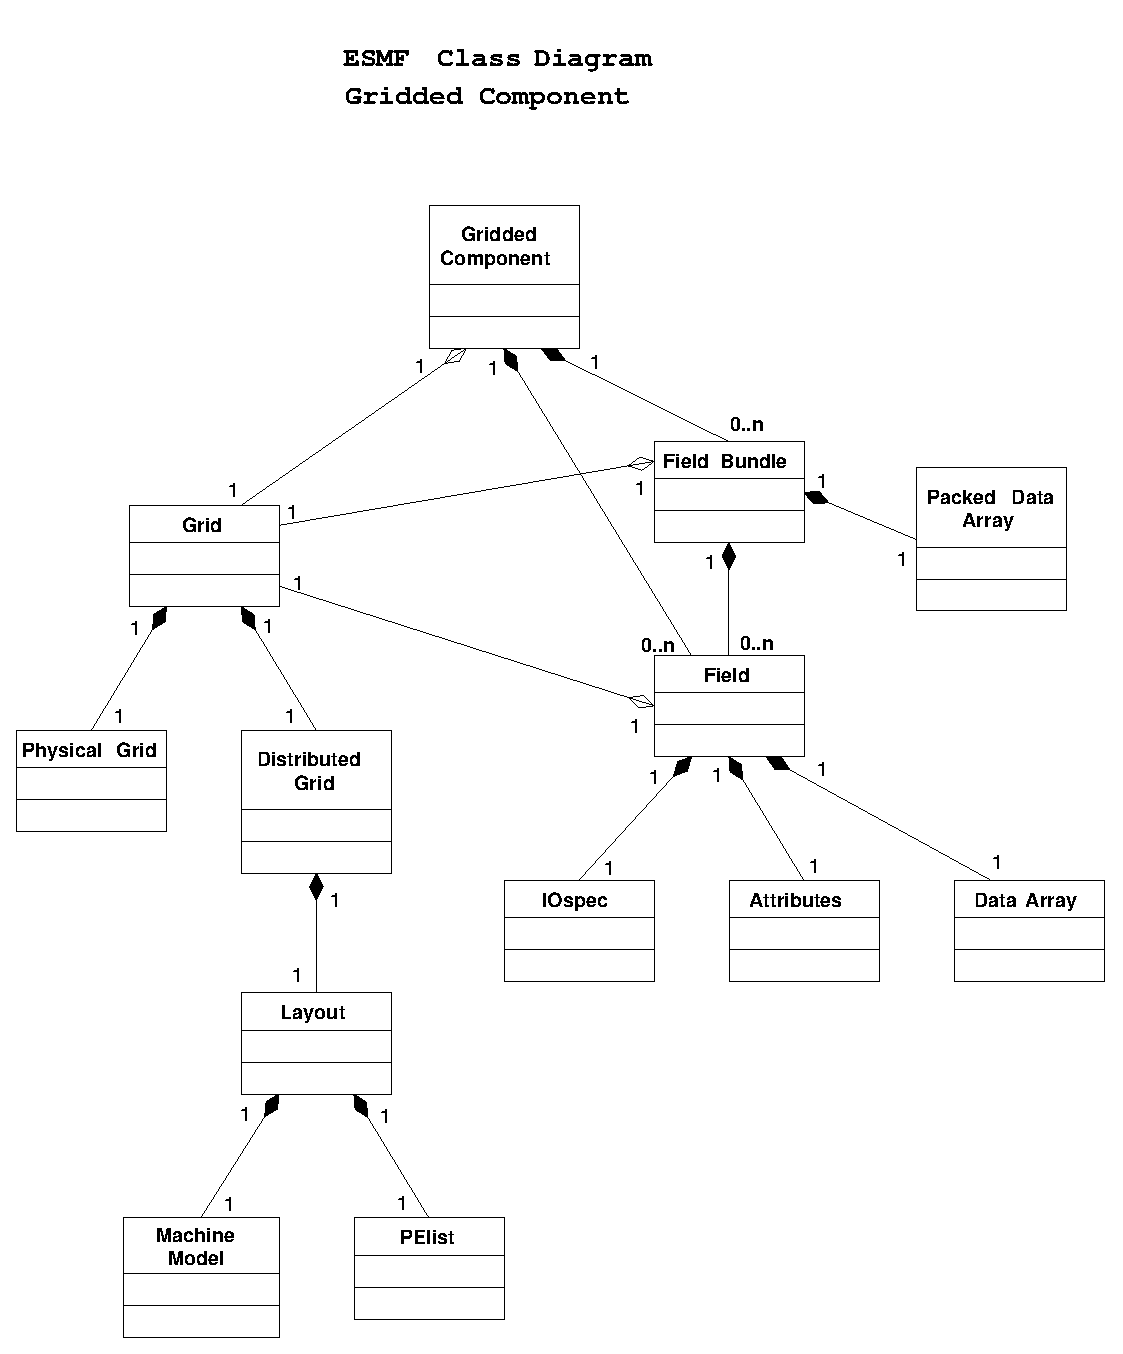
\includegraphics{ESMF_DataStructureHierarchy.eps}}

All objects above are based on the object below.  Attributes
can be handled by generic routines, but it is expected that 
higher level objects will supply their own class specific
methods of the ones listed below.

\scalebox{0.70}{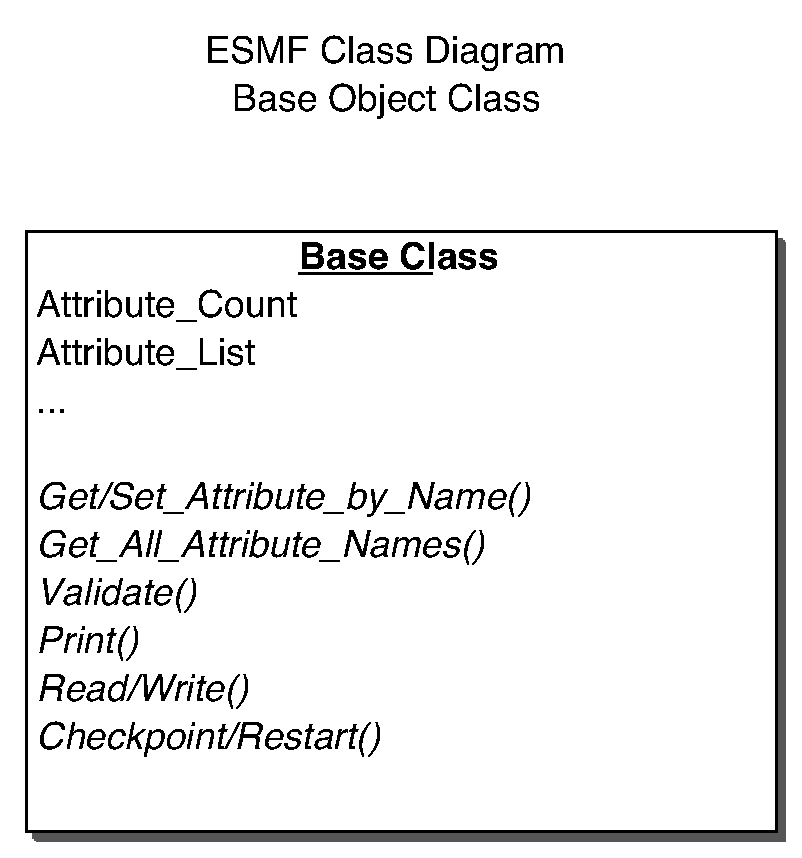
\includegraphics{ESMF_Base.eps}}

Types of components are shown below.

\scalebox{0.70}{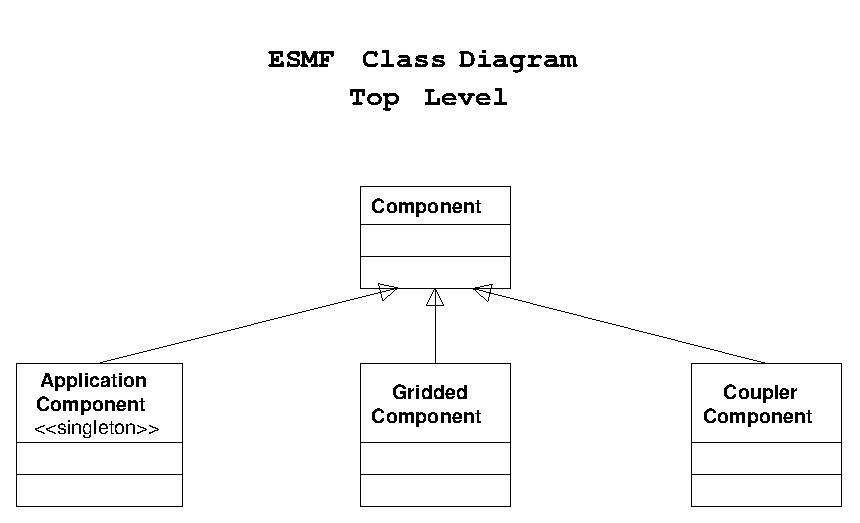
\includegraphics{ESMFTopClassDiagram.eps}}

Coupling diagram.

\scalebox{0.70}{\includegraphics{ESMF_coupler.eps}}

\subsection{Coupling Superstructure}

Below, needs a thorough gutting.

\subsubsection{Component (ESMF\_Comp)} 
\begin{description}
\item [Description] A Component is a functionally related computational entity that represents 
a large system.  
\end{description}

\subsubsection{Application (ESMF\_App)}
\begin{description} 
\item [Description] We define an Application (ESMF\_App) as a special kind of Component 
that is itself composed of a set of sub-Components that interact to form a complete scientific
application.  
\item [Function] The ESMF\_App class is responsible for managing those functions that relate 
to an entire scientific application running under ESMF.  The ESMF\_App initialize method 
must be called at the start of any user application operating under the framework, and
the ESMF\_App finalize method at its end.  At initialization the Application allocates and 
configures any resources needed to run the framework.  The Application also specifies whether 
the system will be brokered using the Registry or not.  The ESMF\_App class can be queried 
for information such as an experiment name, model name, run type (ESMF\_INIT, 
ESMF\_BRANCH, etc.), and for an overall Status.  It can also be queried for
information on any Component that it includes, including its Name, Map, and
Status.
\end{description}

\subsubsection{Coupler Component (ESMF\_Coupler)}
\begin{description}
\item [Description] A Coupler is a specialized type of Component that encompasses all the 
functionality needed to communicate
data between two or more Components. 
\end{description}

\subsubsection{Gridded Component (ESMF\_GComp)} 
\label{sec:gridcomp}
\begin{description}
\item [Description] A Gridded Component is a specialized type of Component that is associated
with a Distributed Grid.  
\end{description}

\subsubsection{Transform (ESMF\_XForm)} 
\begin{description}
\item [Description] A Transform takes one or more physical quantities defined using one set 
of units or representation
and translates them as needed to a different set of units or representation, for example, 
potential temperature
to temperature.  Transform objects are specialized by the application developer.
\item [Function] The Transform class is an abstraction introduced for the
purpose of standardizing high-level coupling interfaces.  It may be overloaded
to take sets of individual Fields or Field Groups.  Methods may include a
separate initialization and run. 
\end{description}

\subsubsection{Layout (ESMF\_Layout)}
\label{sec:layout} 
\begin{description}
\item [Description] A layout is a description of a computational domain that
may describe the decomposition of an Application, a Component, a Field Group, a Field, or 
a Distributed Grid.
If no Layout is specified for an object, it can inherit its layout from an object
higher in the data hierarchy.  
\end{description}

\subsubsection{Distributed Grid (ESMF\_DistGrid)} 

\subsubsection{Field (ESMF\_Field)}
\begin{description} 
\item [Description] A Field represents a single physical field or the components of a 
vector field.  
\end{description}

\subsection{Utility Infrastructure}

\subsubsection{Basic Utilities (ESMF\_BasicUtil)} 
\begin{description}
\item [Description] Utilities that may be utilitized by any other class in the ESMF.  
Collecting these functions into a base-level utility set helps to 
avoid circular referencing.
\item [Function] 
\end{description}

\subsubsection{Basic Communications (ESMF\_BasicComm)}
\begin{description}
\item [Description] This library is a wrapper for MPI and other vendor-supplied 
message passing libraries.
\item [Function] The Basic Communication library provides a generic interface
and efficient communications for the ESMF.  Methods include scatter, gather, send,
receive, synchronize. 
\end{description}

\subsubsection{ (ESMF\_Machine)} 
\begin{description}
\item [Description] The Machine class provides a representation of 
key features of computer hardware and system software.  These
features include memory attributes and configuration, processor type and speed,
interconnect attributes, and system library availability.
\item [Function]
The main purpose of the Machine is to store hardware and system software
information needed by the framework or application programmer in a general
form, but with little abstraction.  This information can be used to perform resource 
allocation, data distribution, and dynamic load balancing.  The Machine can be queried
for platform type(s), number of processors, number of threads, and number of 
nodes.  It may optionally provide information on quantities such as bandwidth and 
latency through active tests.  
\end{description}

\subsubsection{Time Manager (ESMF\_Date, ESMF\_DT)}
\begin{description}
\item [Description] The date and time interval methods in the ESMF provide date
calculations based on a number of different calendars.

\end{description}

















% $Id: ESMF_usage.tex,v 1.9 2002/09/10 18:11:40 cdeluca Exp $

\subsection{Bindings}

The library includes both C/C++ and F90 bindings.  The C/C++ prefix
for procedures and parameters is {\tt ESMC\_} and the F90 prefix is
{\tt ESMF\_}.

\subsection{Object Function Conventions}

To enhance ease of use in the ESMF, naming conventions are
used for common methods such as creation and initialization.

\begin{itemize}
\item{\tt ESM[F/C]\_<Class>New} Allocates a {\it deep} object.  This
  function will allocate space from the heap and may create other
  resources which must be free'd or deallocated.  All items created
  with {\tt New} must be deleted with {\tt Delete} below.  {\tt e.g.
    ESMF\_LogNew}
  
\item{\tt ESM[F/C]\_<Class>Delete} De-Allocates an object created with
  New.  Any transient resources that were created will be cleaned up.
  {\tt e.g. ESMF\_LogDelete}
  
\item{\tt ESM[F/C]\_<Class>Init} Initializes a {\it shallow} object.
  This class of objects does not need to be destructed and is
  guaranteed not to allocate any resources that must be cleaned up.
  {\tt e.g. ESMF\_TimeInit}
  
\item{\tt ESM[F/C]\_<Class>Set<Value>} Sets a given value with the
  class.  The {\tt Value} parameter is decided by the class.  {\tt
    e.g. ESMF\_LogSetState}
  
\item{\tt ESM[F/C]\_<Class>Get<Value>} Gets a given value with the
  class.  The {\tt Value} parameter is decided by the class.  {\tt
    e.g. ESMF\_LogGetState}
  
\item{\tt ESM[F/C]\_<Class>SetConfig} This function takes a list of
  resorces as defined in the resource section the class.  Some class
  may not have resources and this function has no meaning.  The
  function allows a user to set multiple resources with one function
  call.  {\tt e.g. ESMF\_LogSetConfig}
  
\item{\tt ESM[F/C]\_<Class>GetConfig} This function takes a list of
  resorces as defined in the resource section the class.  Some class
  may not have resources and this function has no meaning.  The
  function allows a user to get multiple resources with one function
  call.  {\tt ESMF\_LogGetConfig}
  
\item{\tt ESM[C]\_<Class>Construct} This function fills initializes an
  object with valid data.  This function is called by both the {\tt
    Init} and {\tt New} functions.  Depending on the type of object
  this function may or may not allocate resources that need to be
  freed.
  
\item{\tt ESM[C]\_<Class>Destruct} This function cleans up any
  resources that were created in the {\tt Construct} method.

\end{itemize}

\subsection{Constraints}

The library design imposes some constraints on the user:

\begin{itemize}
\item {\it No direct access of Fortran derived types.} Elements of
  Fortran derived types are private.
  
\item{\it All types should be initialized.} In order to provide
  consistent argument checking and to increase the overall robustness
  of the library, a user should call one of the {\tt Init}
  routines before using the library's Fortran derived types, or the
  {\tt Construct} routine before using its C/C++ classes.  A {\tt
    New} routine is provided for C/C++ if dynamic memory
  allocation is desired.

\end{itemize}

\subsection{Error Handling}

All C/C++ procedures return an integer error code.  All F90 procedures have 
an optional integer return code argument (with the exception of a select few
functions that use {\tt stdargs}).  Return codes are translated 
into error descriptions using the methods: 

\begin{verbatim}
    void ESMC_ErrPrint(int rc)

    subroutine ESMF_ErrPrint(rc)  
    integer, intent(in), optional :: rc
\end{verbatim}

A return code of {\tt ESM[F/C]\_SUCCESS} indicates that an 
operation executed without errors.

The user can currently choose from two different error handlers.
{\tt ESM[F/C]\_ERR\_RETURN} will simply return from a routine in which an error 
is identified, without printing an error description.
{\tt ESM[F/C]\_ERR\_EXIT} will print a detailed error description including
file, function name, and line number, and will then terminate execution
(this is a simple exit, not an {\tt MPI\_ABORT}).  These handlers are set 
using the methods: 
\begin{verbatim}
    void _ErrHandlerSetType(ESM[F/C]_ErrHandlerType type)

    subroutine ESM[F/C]_ErrHandlerSetType(type)
    integer, intent(in) :: type
\end{verbatim}

The intent is to provide an error handling system in which
users can choose from a variety of handlers or supply their own.










\newpage
\begin{htmlonly}
\addcontentsline{toc}{part}{Superstructure}
\end{htmlonly}
\part{Superstructure}
\label{part:Superstructure}

%\subsection{Components and Control}

%\subsection{Coupling}
\section{ESMF Superstructure:  Coupling and Control}
\label{sec:superclasses}

\subsection{Introduction}

In this section, we describe the classes involved in the ESMF superstructure, 
their relationships, and typical action sequences for component interactions.

\subsection{Design Goals and Considerations}

One of the primary goals of the ESMF project is to increase interoperability
across a range of Earth system modeling components.  Initially these 
components will be large scale, such as land models, ocean models, 
and data assimilation systems.  Earth system research 
often requires that such components be coupled together in multiple
configurations.  We identify user-supplied components discretized on grids with 
a {\tt Gridded Component} class, and the software used to couple them together
with a {\tt Coupler Component} class.  

As the framework evolves, we plan to utilize ESMF coupling services for 
smaller-scale tasks within model components, such as the transformation of 
data between the 
physics and dynamics in a spectral atmospheric model, and the creation 
of nested higher resolution regions within a coarser grid.  The goal is 
to couple components at varying scales both flexibly and efficiently.  
Our strategies for accomplishing this are as follows.

We aim to keep the coupling specification entirely external 
to {\tt Gridded Component}s involved in an interaction, which makes it easier 
for the same {\tt Gridded Component} to be reconfigured for a different 
coupled application.
This is closely related to the ``mediator'' strategy for handling complexity in 
software that requires many inter-component interactions (see Section~\ref{sec:oop}).  
We avoid excessive complication in the {\tt Coupler Component} by limiting
its responsibility; the {\tt Coupler} component does not instantiate 
gridded components, schedule, or run them.  These tasks are performed
by an {\tt Application Component} or other parent component (see 
Section~\ref{sec:controlflow}).

The ability to remap to adapt to different computing platform sizes 
and characteristics is essential for performance portability.
Where their physics content permits
{\tt Gridded Component}s can be configured for
sequential or concurrent execution without changes to the {\tt Gridded 
Component} code.  Changes to {\tt Coupler} and/or {\tt Application Component} code are likely to 
be required (see Section~\ref{sec:scoping}). This is possible because 
the {\tt Gridded Component} uses the infrastructure layer to abstract communication
protocols such that a {\tt Gridded Component} looks the same on all
platforms. Additionally, the superstructure layer ensures that a {\tt Gridded
Component} can be created to execute concurrently or sequentially through the
manipulation of PE lists.

The ability to overlap computation with communication is also essential for
performance.  We facilitate this by enabling the user to initiate data 
sends during {\tt Gridded Component} execution, as soon as the data is ready.

To further increase efficiency, data may be sent between components without 
needing to be sent to a {\tt Coupler} as an intermediate step (see
Section~\ref{sec:dataflow}).

It is not necessary to create return points from 
within the time iteration loop of a {\tt Gridded Component}.  This reduces the
amount of work application groups will need to perform to adopt the 
framework.

There is considerable interest in evolving the ESMF into a more comprehensive
Problem Solving Environment (PSE).  The systematized approach to component 
scheduling we have adopted will enable a layer of tools for application 
configuration to be added to the architecture in the future.

\subsection{Classes and Scoping}
\label{sec:scoping}
There are restrictions on how ESMF components within an Earth system application 
can be scoped on a parallel platform.  There is only one {\tt Application Component} 
defined for any application; it initially allocates resources and tracks 
application-wide information. 
The {\tt Application Component} must be instantiated on 
any {\tt Decomposition Elements}\footnote{In ESMF {\tt Decomposition Elements} are the
basic abstraction that provides platform neutral parallelism, they are discussed in detail
in Section~\ref{sec:progmodel}} or {\tt DE}s on 
which other components
within the application are defined.  This is true whether the 
application consists of a single executable or multiple 
executables.  

An ESMF coupled application typically involves an {\tt Application Component} 
containing two or more {\tt Gridded Component}s that require an 
inter-component data exchange, and one or more {\tt Coupler 
Component}s.  However, any parent component that contains the appropriate 
subcomponents can manage their execution and coupling.  ESMF thereby
supports applications consisting of a hierarchy of coupled systems.

A {\tt Coupler Component} must be instantiated on any {\tt DE}s on which components
it will couple are defined.  This is consistent with an architectural
model in which communication is handled internal to components, and all
inter-component interactions are local (see Section~\ref{sec:strategies}).  
It is possible for
some portions of the functionality of a component to be restricted to
a subset of the {\tt DE}s over which the component is defined.  For example, 
it may be computationally efficient for the computation of interpolation
weights to occur on a set of {\tt DE}s not being used by any {\tt Gridded 
Components}
in the application.  The {\tt Coupler} might define a subcomponent on 
those {\tt DE}s specifically to handle the interpolation function.

A {\tt Gridded Component} may exist across all {\tt DE}s in an {\tt Application}.  
When a set of {\tt Gridded  Component}s and a {\tt Coupler} all execute in sequence on 
the same set of {\tt DE}s and are contained within an application running 
as a single executable we have a sequential execution SPMD configuration.  

Within an application, a {\tt Gridded Component} may also reside on 
a subset of {\tt DE}s.  These {\tt DE}s may wholly coincide with, be wholly 
contained within or wholly contain another component.  

It is possible for ESMF applications to contain some component sets
that are executing sequentially and others that are executing concurrently.
We might have, for example, atmosphere and land components instantiated 
on the same set of 
{\tt DE}s and running as one executable, ocean and sea ice 
components instantiated on a separate set of {\tt DE}s and running as 
another executable, and a {\tt Coupler} and {\tt Application Component} 
instantiated across all {\tt DE}s.

Figure~\ref{fig:couplerscaling} illustrates scoping of components
in a coupled, hierarchically structured application.  At the top level, 
a climate application consists of atmosphere and ocean components 
instantiated on mutually exclusive {\tt DE} sets.  These components communicate 
via an atmosphere/ocean {\tt Coupler} defined on the union of their {\tt DE}s.  
Scheduling is controlled by an {\tt Application
Component} which is also defined across all {\tt DE}s.  The atmosphere component
is similarly structured as a coupled application.  It consists of a 
physics component and a dynamics component, which are both distributed
across all the atmospheric {\tt DE}s.  A physics/dynamics {\tt Coupler} controls
the data transpose between these subcomponents.  In this case, the
atmospheric component rather than the highest level application component
controls the coupling sequence.  

\begin{figure}
\caption[{Scoping of Components in a Coupled Application}]{A coupled
application may itself be composed of other coupled systems.}
\label{fig:couplerscaling}
\begin{center}
\scalebox{0.7}{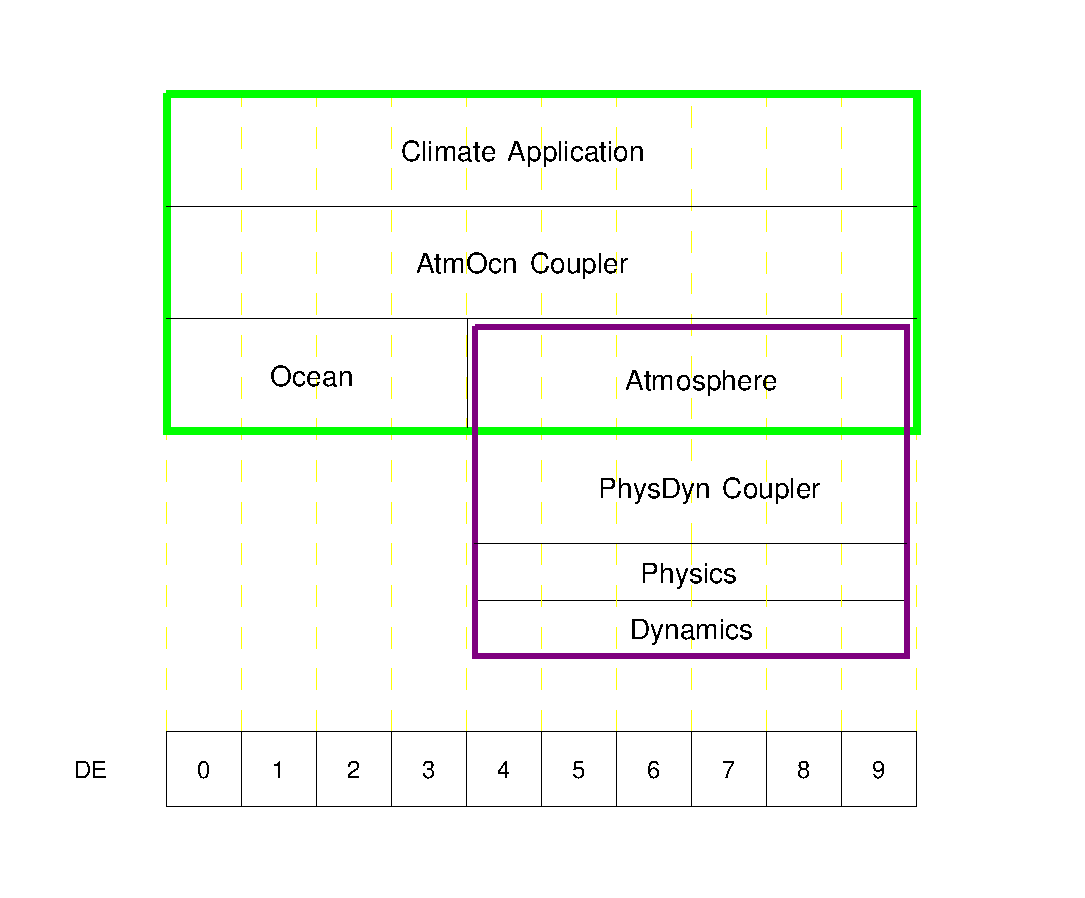
\includegraphics{CouplerScaling.eps}}
\end{center}
\end{figure}


\subsection{Flow of Control}
\label{sec:controlflow}
{\tt Gridded components} have few responsibilities with respect to coupling
to other components.  They do not need to keep track of the data needed
by other components or to provide methods for inter-component 
grid transformations or transfers of data.  They {\it are} responsible for 
providing a description of all of the fields and data they
can export to other components, and for similarly providing a description 
of the data they require in order to run.  These descriptions are
embodied in the {\tt ESMF\_State} class, and the kind of data that they 
represent is identified by the {\tt type} attribute of that class, which can
have an {\tt ESMF\_IMPORT} or {\tt ESMF\_EXPORT} value.  The {\tt State} class
includes metadata information, actual pointers to data 
locations, and default criteria for data validation.  The last of these in its
simplest form may be a bit that is set when data is ready for use.  The ESMF 
will provide methods that enable a user to add or remove fields and data from 
{\tt State}s.  

A {\tt Coupler Component} produces a specification of the sequence of 
operations that are necessary to effect communication between components, 
both scientific and computational, generic and user-defined.  The {\tt Coupler} 
may be called directly, or it may return a set of {\tt Transform} objects to 
the {\tt Application} or parent.  Each {\tt Transform} has a
function pointer to a coupling operation and may be bundled with 
associated data, information about coupling frequency, and 
data validation criteria. With sequentially executing components the {\tt Coupler}
may be invoked directly from within the timestepping loop.  For concurrently executing
components the {\tt Coupler} may initially generate a set of {\tt Transforms}, which 
are passed at the application level to individual components.  These components
can execute the {\tt Transforms} without needing to return control to the 
{\tt Application}.

The {\tt Application} or parent component initiates the coupling and manages 
its scheduling.  It is responsible for instantiating the {\tt Gridded Component}s
that are exchanging data and instantiating the {\tt Coupler}, for setting up the desired 
sequencing, and making the calls to the methods of the components and 
{\tt Coupler} that effect the exchange.  The parent may partition the 
transforms
for execution among the {\tt Gridded Component}s and the {\tt Coupler}, so that, for 
example, a data send or coupling transformation can occur while a {\tt Gridded 
Component} is executing, without a need for the component to return to the
parent level.  
To disable or rearrange the coupling sequence, a different set of function
pointers can be passed to the component.

The {\tt ESMF\_StateTransform} call executes a {\tt Transform} 
within a {\tt Gridded Component}.  It takes as arguments a
{\tt Transform} object and the component's import or export {\tt State}.  
For {\tt Transform}s that initiate non-blocking sends, a {\tt ESMF\_StateTransformComplete} 
call can check that data  buffers are available for reuse.  This 
call takes the initiated {\tt Transform} object as an argument.

The {\tt ESMF\_StateValidate} call evaluates whether a component's 
import {\tt State} is ready for use.  It may check the entire {\tt State} or 
a specified subset.

\subsection{Flow of Data}
\label{sec:dataflow}
The design choices we have made enable the user to configure ESMF
applications so that data is transferred from one component to another, 
without requiring that it first be sent via message passing to a
{\tt Coupler} (or even necessarily
copied).  This is likely to be the most efficient way of performing 
inter-component coupling when the components are instantiated on different
{\tt DE} sets.  However, if desired, an application can also be configured so that
data from a source component is sent to a distinct set of {\tt Coupler} 
{\tt DE}s for processing before being sent to its destination.

\section{Examples}

Here we describe a number of example scenarios of ESMF usage. The examples are
described in text and illustrated using UML sequence diagrams. In these diagrams
The vertical axis is time, positive
downward, and the horizontal axis shows the objects that are involved in the
exchange.  Arrowed lines to text boxes mean that the source of the arrow has
created the object in the box.  Solid lines to the start of a vertical
box indicate a method call.  Dashed lines indicate a return.
The overall flow of execution is partitioned into four stages in this
discussion, {\it Create Sequence}, {\it Configure Sequence}, {\it Run Sequence}
and {\it Termination Sequence}.
 
\subsection{Create Sequences}

An ESMF application begins with the creation of components. The
three sequence diagrams in figures \ref{fig:ApplicationComponentCreate}, 
\ref{fig:CouplerComponentCreate} and 
\ref{fig:GriddedComponentCreate} show the
component creations steps for different types of component.


\subsubsection{Application Creation}
Figure \ref{fig:ApplicationComponentCreate} shows the sequence associated with
creation of components from an {\tt Application Component}. In the diagram,
creation of child components executes concurrently. The application component
proceeds through three phases which are serialized with respect to one another.
First the application component creates a registry object for this application,
next it creates two gridded components, finally it creates two coupler
components for transporting and translating data between gridded components.
The actions within each phase can be parallelized, however, the phases
themselves execute sequentially.
\begin{figure}
\caption[{Application Component Create}]
{The UML sequence for application component creation}
\label{fig:ApplicationComponentCreate}
\scalebox{1.0}{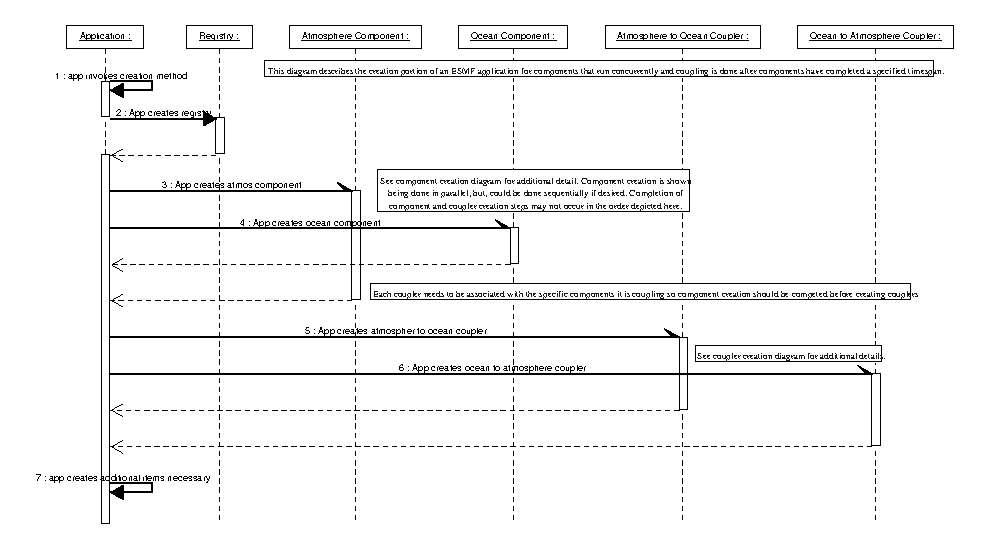
\includegraphics{CreateAppDiagram.eps}}
\end{figure}


\subsubsection{Coupler Component Creation}
Figure \ref{fig:CouplerComponentCreate} shows the sequence associated
with creation in a {\tt Coupler Component}. The key steps involved are
the creation of import and export Xpackets that respectively hold inputs and
outputs of the coupler component. Coupler component creation may also involve
internal, coupler component specific initialization and, additionally,
registering the coupler components presence with the global registry entity.

\begin{figure}
\caption[{Coupler Component Create}]
{The UML sequence for coupler component creation}
\begin{center}
\label{fig:CouplerComponentCreate}
\scalebox{1.0}{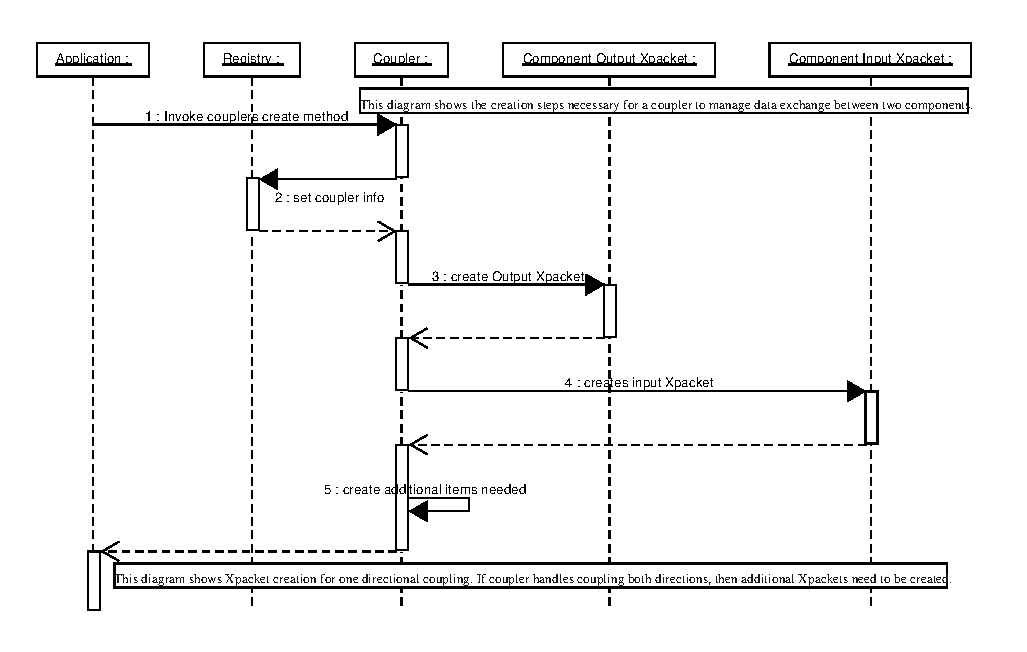
\includegraphics{CreateCouplerDiagram.eps}}
\end{center}
\end{figure}

\subsubsection{Gridded Component Creation}
Figure \ref{fig:GriddedComponentCreate} shows the sequence associated with
creation in a {\tt Gridded Component}. A key step in Gridded Component
creation is the creation of import and export states for transferring 
data to and from other components. In addition there may be component
specific computation that is executed during creation as well as execution
of a registration function to register the component in the global registry.

\begin{figure}
\caption[{Gridded Component Create}]
{The UML sequence for gridded component creation}
\begin{center}
\label{fig:GriddedComponentCreate}
\scalebox{1.0}{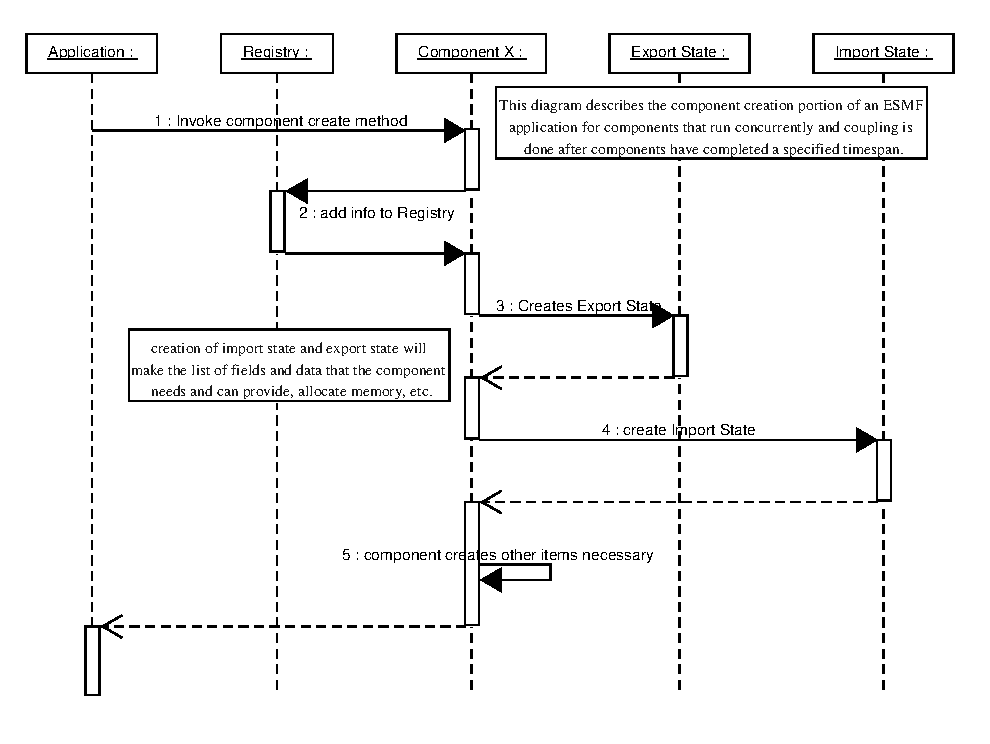
\includegraphics{CreateComponentDiagram.eps}}
\end{center}
\end{figure}

\subsection{Configure Sequences}
Following component creation a configuration step is invoked. This step
invokes component specific logic that is responsible for setting the component
initial state. Figures \ref{fig:ApplicationComponentConfigure}, 
\ref{fig:CouplerComponentConfigure} and 
\ref{fig:GriddedComponentConfigure} show the component
configuration sequences for different types of component.

\subsubsection{Application Component Configuration}
Figure \ref{fig:ApplicationComponentConfigure} shows the sequence associated 
with configuration in an {\tt Application Component}. The sequence begins 
with internal configuration of the application component. The application
component then invokes the configuration methods for the gridded components
within its scope and for the coupler components within its scope.
Gridded component configuration completes before coupler component
configuration in invoked. In the example shown in the figure configuration
for the individual gridded components executes concurrently as does 
configuration for the individual coupler components.


\begin{figure}
\caption[{Application Component Configuration}]
{The UML sequence for application component configuration}
\begin{center}
\label{fig:ApplicationComponentConfigure}
\scalebox{1.0}{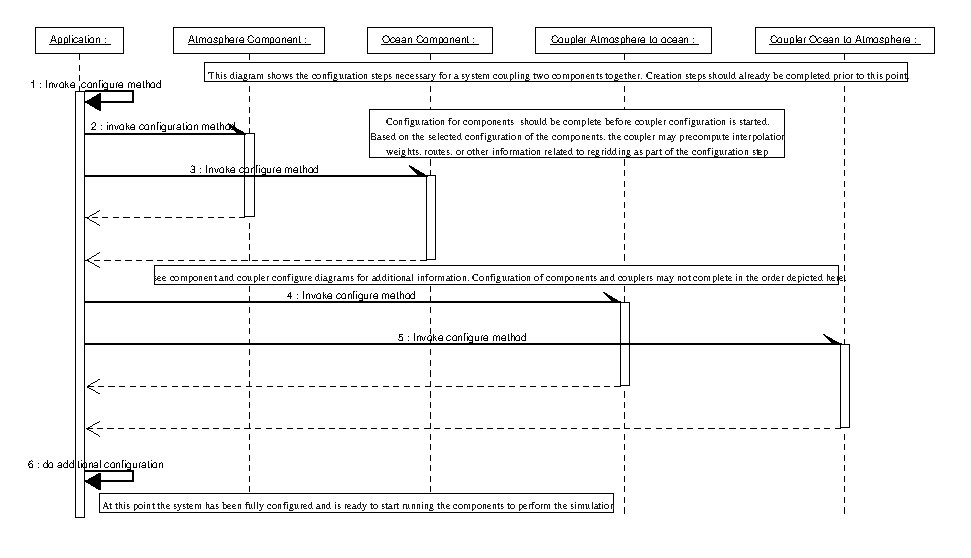
\includegraphics{ConfigureAppDiagram.eps}}
\end{center}
\end{figure}

\subsubsection{Coupler Component Configuration}
Figure \ref{fig:CouplerComponentConfigure} shows the sequence associated 
with configuration of a {\tt Coupler Component}. A coupler components
configuration method is invoked from its parent
component (the {\tt Application Component} in the case of
figure \ref{fig:CouplerComponentConfigure}). Once invoked the method
is responsible for initializing the coupler's import and export states 
to a known, valid condition. Additional computation, specific to a particular
coupler component, may also be included. This could include precalculation
of interpolation weights that are repeatedly used in a specific regridding
operation.

\begin{figure}
\caption[{Coupler Component Configuration}]
{The UML sequence for coupler component configuration}
\begin{center}
\label{fig:CouplerComponentConfigure}
\scalebox{1.0}{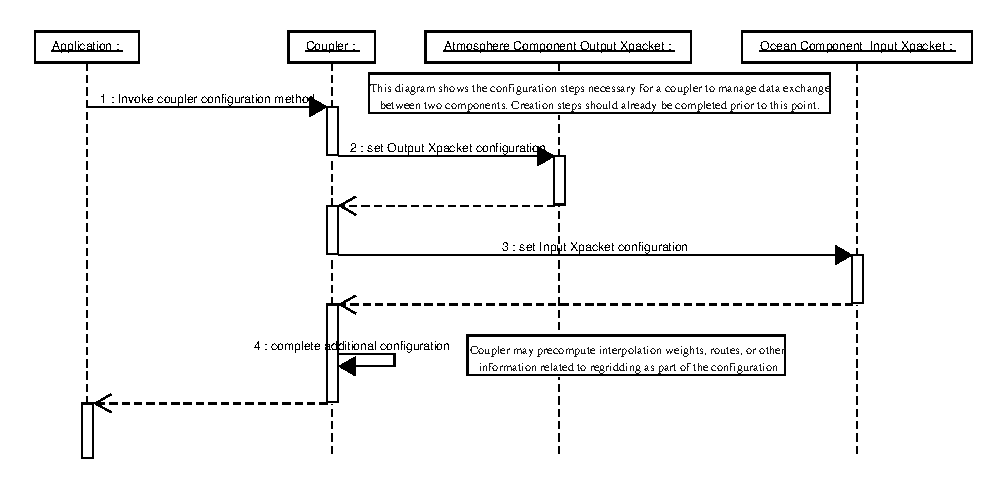
\includegraphics{ConfigureCouplerDiagram.eps}}
\end{center}
\end{figure}

\subsubsection{Gridded Component Configuration}
Figure \ref{fig:GriddedComponentConfigure} shows the sequence associated 
with configuration in a {\tt Gridded Component}. The component configuration
method is invoked from the parent component (the {\tt Application Component}
in figure \ref{fig:GriddedComponentConfigure}). Once invoked the configuration
stage is responsible for configuring the import and export states for the 
component to a known, valid status. Component configuration may also include
specialized configuration steps specific to that particular
component. On completion the configuration method returns to the
parent component.

\begin{figure}
\caption[{Gridded Component Configuration}]
{The UML sequence for gridded component configuration}
\begin{center}
\label{fig:GriddedComponentConfigure}
\scalebox{1.0}{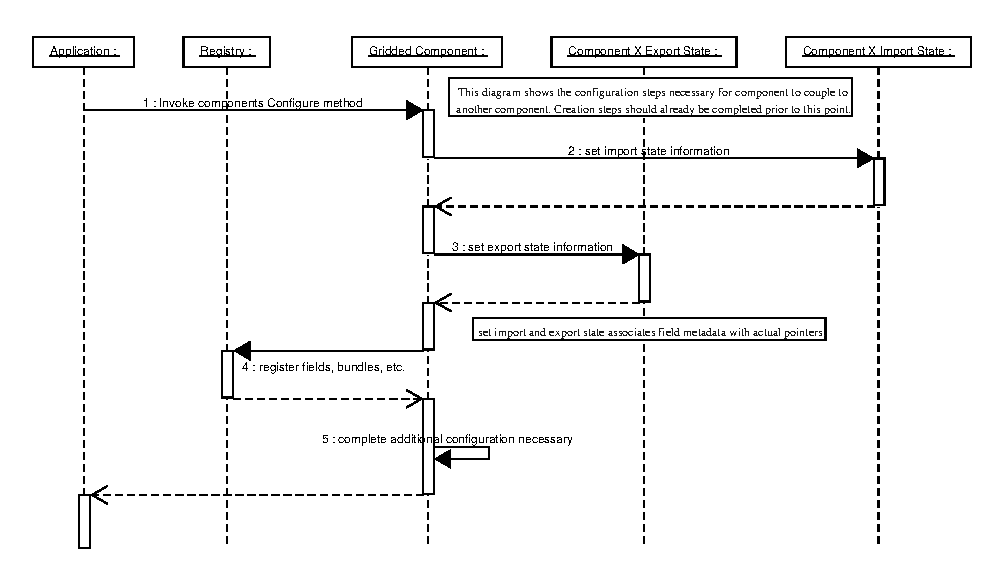
\includegraphics{ConfigureComponentDiagram.eps}}
\end{center}
\end{figure}

\subsection{Run sequences}
This section shows sequence diagrams for a number of different run scenarios.
For each sequence, the preceding component creation and component configuration 
phases are omitted for clarity.

\subsubsection{Concurrent coupled atmosphere ocean sequence}

Figure \ref{fig:RunApplicationDiagram} shows the sequence of actions involved
in running an atmosphere ocean coupled system. In the example the
coupling is two-way, with the ocean receiving data from the atmosphere and 
sending data back to the atmosphere.  Atmosphere and ocean components are 
configured for concurrent execution.

\begin{figure}
\caption[{Basic Run Application}]{A prototypical UML sequence for a basic Run Application stage.\\}
\label{fig:RunApplicationDiagram}
\scalebox{1.0}{\includegraphics{runApplicationDiagram.eps}}
\end{figure}

Following {\tt Application Component} startup (and coupler and component
creation and configuration) the run methods of components are 
invoked. An example of this procedure is illustrated in figure 
\ref{fig:RunApplicationDiagram}. In 
the example given, the {\tt Application Component} invokes the run method of 
the of the Atmosphere and Ocean gridded components concurrently. The 
application 
component then waits until these stages are complete before it invokes the 
coupler components run methods. The coupler components
take export states from the atmosphere and ocean respectively. 
The coupler components are invoked to run concurrently with one another. Before iterating 
onto the next time step the {\tt Application Component} selectively invokes the 
checkpoint/restart methods of the Ocean and Atmosphere components, again 
concurrently. Finally the {\tt Application Component} evaluates whether
to exit or whether to return to the start of the run loop for subsequent 
iteration.

\subsubsection{Sequential Components Run Sequence}

Figure \ref{fig:SequentialComponentsRunSequence} shows the UML sequence
for a multi-component application in which components execute serially
with respect to one another. Each component may itself be a parallel
computation, however, execution of methods in one component do not overlap 
with execution of methods in other component in this example.
For an individual object the event sequence mirrors the procedure in 
figure \ref{fig:RunApplicationDiagram}. However, in the sequential
case only one event is active at any time.
\begin{figure}
\caption[{Sequential Component Run}]{Sequence for serial multi-component
application.\\}
\begin{center}
\label{fig:SequentialComponentsRunSequence}
\scalebox{1.0}{\includegraphics{RunAppSequencialDiagram.eps}}
\end{center}
\end{figure}

\subsubsection{Subcomponent Run Sequence}
Figure \ref{fig:SubcomponentRunSequence} shows the execution of an
application with components and subcomponents. In this case the 
two components (atmospheric physics and atmospheric dynamics) are 
subcomponents
of a parent atmosphere component. This configuration requires that extra 
coupler components be employed. These map between import and export states of 
the physics and dynamics components within the the scope of the
parent atmosphere component. In this scenario the sequencing of
subcomponents is controlled by their parent (the atmosphere component)
and not by the application component.

\begin{figure}
\caption[{Subcomponent Run}]{Sequence for component and subcomponent
application.\\}
\begin{center}
\label{fig:SubcomponentRunSequence}
\scalebox{1.0}{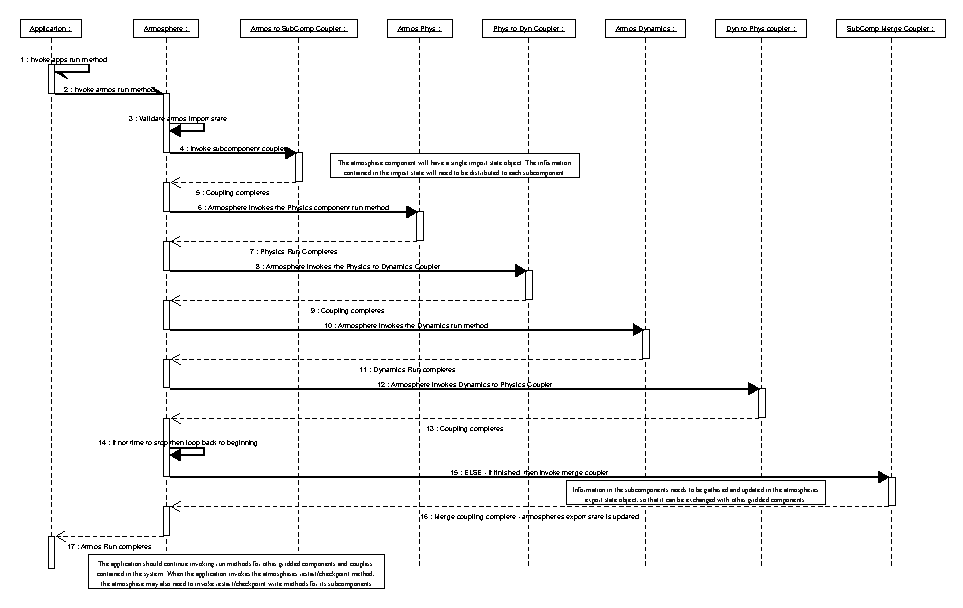
\includegraphics{subcomponentCoupling.eps}}
\end{center}
\end{figure}

\subsubsection{Ensemble Run Sequence}
Figure \ref{fig:EnsembleComponentsRunSequence} shows an ensemble scenario
in which multiple instances of the same component execute in parallel.
The run sequence is driven from the application component. However,
an extra level of coupling indirection is required. This is provided by a
coupler component that merges (in some user defined manner) the export
state of multiple ocean components. The output from this coupler
component is then passed to a coupler component that transforms from an
ocean export state to an
atmosphere component import state.
\begin{figure}
\caption[{Ensemble component Run}]{Sequence for ensemble components
application scenario.\\}
\begin{center}
\label{fig:EnsembleComponentsRunSequence}
\scalebox{1.0}{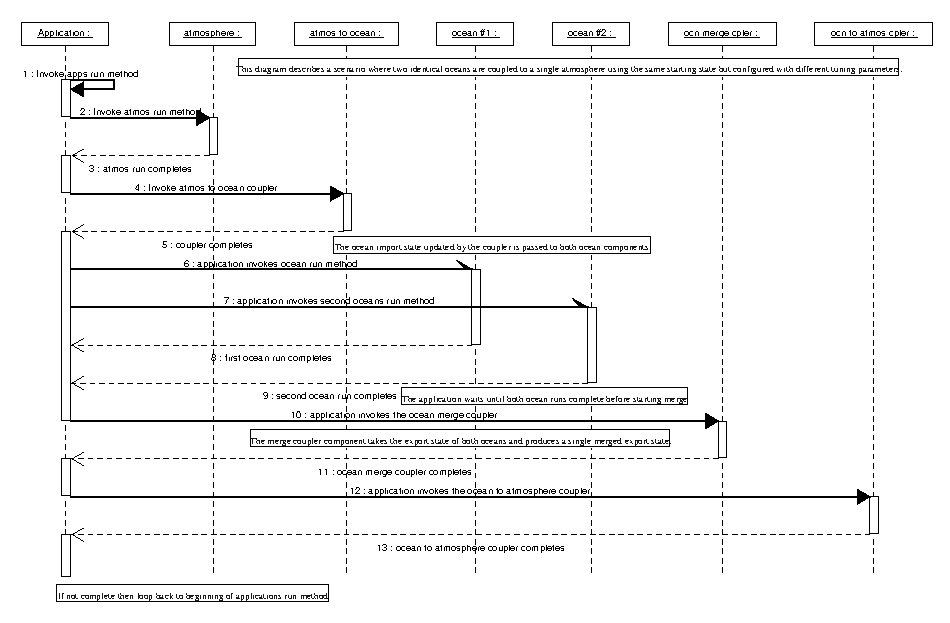
\includegraphics{runMergedApplicationDiagrams.eps}}
\end{center}
\end{figure}

\subsubsection{Ensemble Coupler Component Run Sequence}
Figure \ref{fig:EnsembleComponentsCouplerRunSequence} shows the
{\tt Coupler Component} run sequence in an ensemble scenario. The sequencing
illustrated is invoked from the application component. It proceeds by
first merging two ocean import states into a composite form. The composite
form then serves to update a merged ocean export state that is
configured for import into an ocean-to-atmosphere coupler component 
(labeled {\tt ocn to atmos cpler:} in the figure).
\begin{figure}
\caption[{Ensemble Coupler Run}]{Sequence for ensemble coupler
scenario.\\}
\begin{center}
\label{fig:EnsembleComponentsCouplerRunSequence}
\scalebox{1.0}{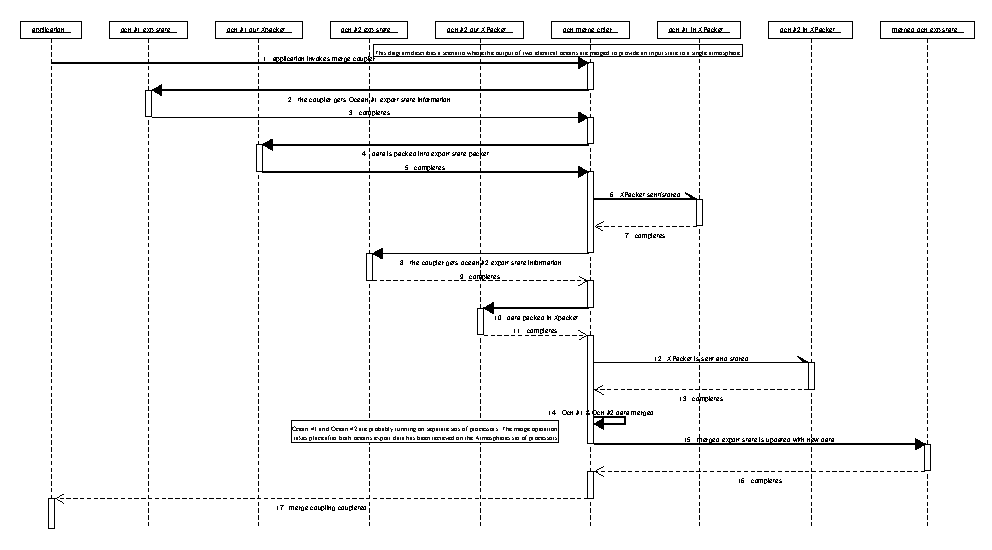
\includegraphics{runMergedCouplerDiagram.eps}}
\end{center}
\end{figure}

\subsubsection{Gridded Component Run Sequence}
Figure \ref{fig:GriddedComponentsRunSequence} shows the internal sequence
that a typical gridded component run method executes. This sequence, 
executed when the components run method is invoked,
consists of decoding and parsing the import state, ''stepping forward'' the 
components internal state, and setting an appropriate export state. The 
component then returns to the parent level.
\begin{figure}
\caption[{Sequence in a Component Run}]{Sequence for a component
run stage.\\}
\begin{center}
\label{fig:GriddedComponentsRunSequence}
\scalebox{1.0}{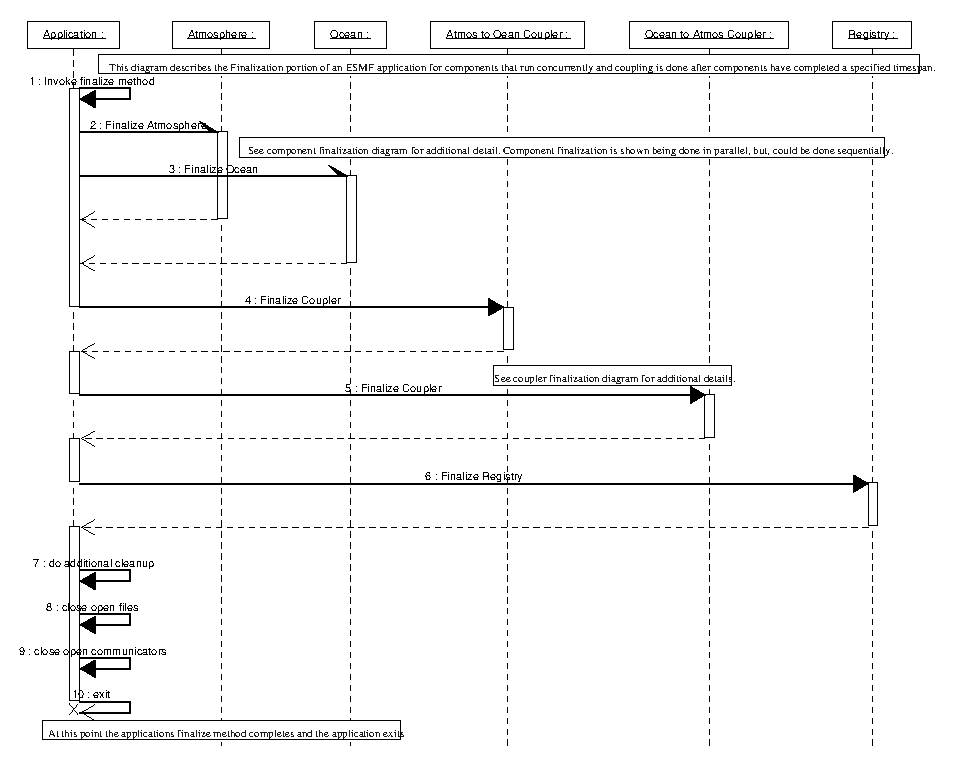
\includegraphics{RunComponentDiagram.eps}}
\end{center}
\end{figure}

\subsubsection{Coupler Component Run Sequence}
Figure \ref{fig:CouplerComponentsRunSequence} shows the internal sequence
that a typical coupler component run method executes. After invocation
from the parent level, this sequence consists
of acquiring, decoding and parsing the export state from another component.
The state is then transformed through regridding and other conversion
procedures. The transformed state is then posted as the import state
for another component and flow returns to the parent component.
\begin{figure}
\caption[{Coupler Component Run Sequence}]{Sequence for a coupler component
run stage.\\}
\begin{center}
\label{fig:CouplerComponentsRunSequence}
\scalebox{1.0}{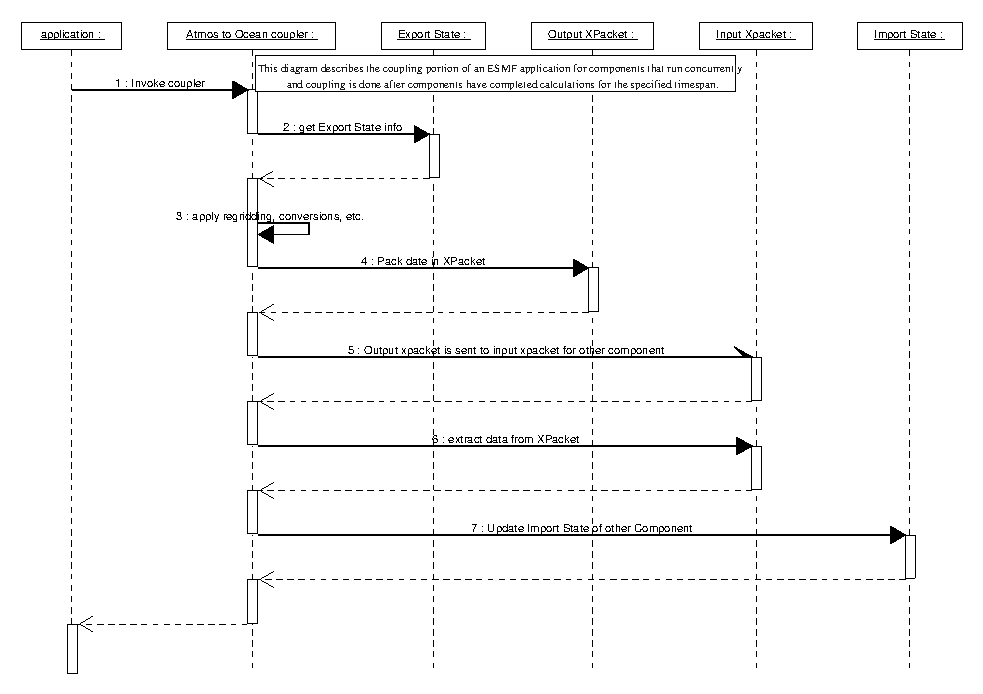
\includegraphics{RunCouplerDiagram.eps}}
\end{center}
\end{figure}

\subsection{Finalize Sequence}
Shut down of an ESMF application follows a regular sequence for each component
type. Figures 
\ref{fig:ApplicationFinalizeSequence}, 
\ref{fig:CouplerFinalizeSequence} and 
\ref{fig:GriddedComponentFinalizeSequence} show the shut down sequence for 
{\tt Application Components}, {\tt Coupler Components} and {\tt Gridded Components} respectively.
\subsubsection{Application Finalize Sequence}

Figure \ref{fig:ApplicationFinalizeSequence} shows the termination sequence
for an {\tt Application Component}. This sequence is executed at
the end of an ESMF application. The sequence consists of an invocation
of the application destroy method which then invokes the destruction methods 
of all the application component's child components. After the child 
components are destroyed the registry object and any other high-level 
structures are also destroyed.

\begin{figure}
\caption[{Application Finalize}]{Sequence for finalizing an application
component.\\}
\begin{center}
\label{fig:ApplicationFinalizeSequence}
\scalebox{1.0}{\includegraphics{FinalizeAppDiagram.eps}}
\end{center}
\end{figure}

\subsubsection{Coupler Finalize Sequence}
Figure \ref{fig:CouplerFinalizeSequence} shows the termination sequence in
a {\tt  Coupler Component}. The sequence is initiated by the parent 
component (in this example the {\tt Application Component}). Upon 
initiation a {\tt Coupler Component} destroy method will delete
the import and export state objects it instantiated at creation and
also perform file and network I/O cleanup operations.
Flow then returns to the parent component.
\begin{figure}
\caption[{Coupler Finalize}]{Sequence for finalizing a coupler component}
\begin{center}
\label{fig:CouplerFinalizeSequence}
\scalebox{1.0}{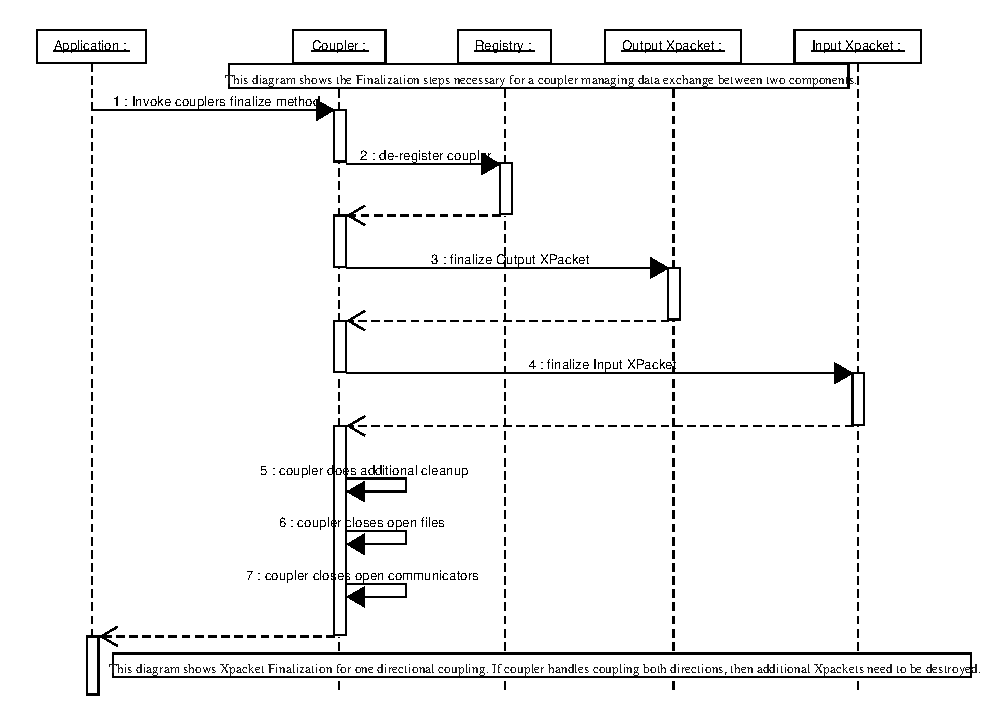
\includegraphics{FinalizeCouplerDiagram.eps}}
\end{center}
\end{figure}

\subsubsection{Gridded Component Finalize Sequence}
Figure \ref{fig:GriddedComponentFinalizeSequence} shows the termination 
sequence in a {\tt Gridded Component}. After being invoked from the
its parent component a gridded component finalize method destroys
export state and import state objects it created along with any
internal structures it has created. Then file and network I/O objects
are closed. Finally flow returns to the parent component.
\begin{figure}
\caption[{Gridded Component Finalize}]{Sequence for finalizing a gridded component}
\begin{center}
\label{fig:GriddedComponentFinalizeSequence}
\scalebox{1.0}{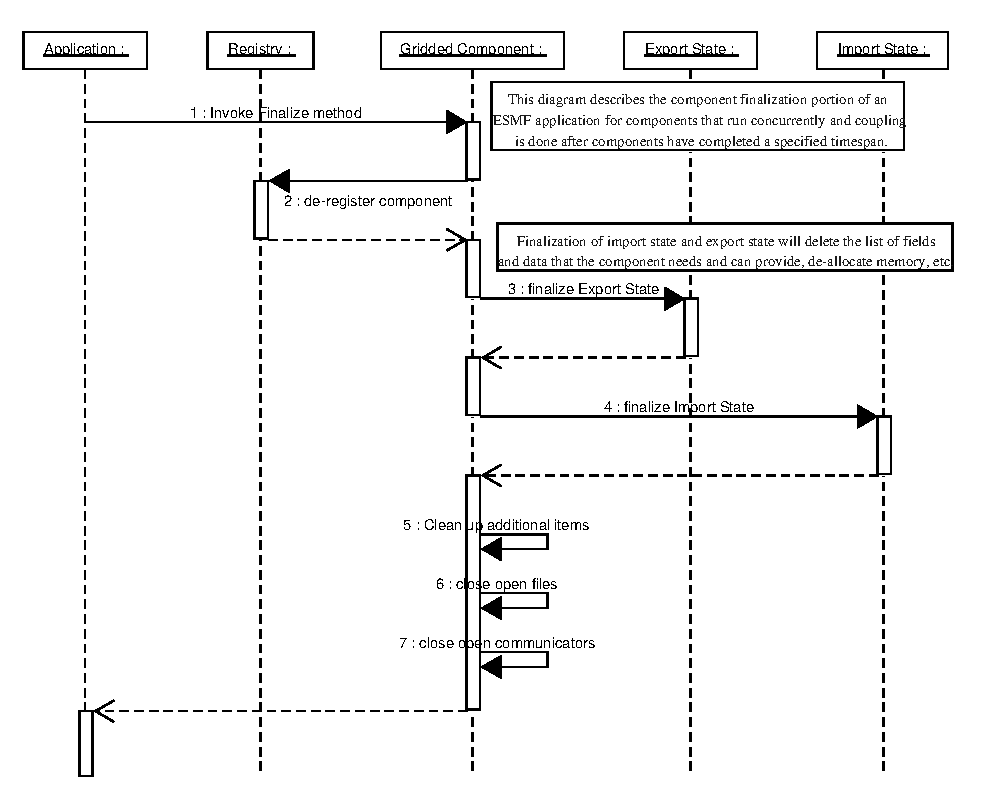
\includegraphics{FinalizeComponentDiagram.eps}}
\end{center}
\end{figure}

\section{Superstructure Class Descriptions}

The following are brief descriptions of the objects involved in the
ESMF superstructure. The relationship between the key component classes
({\tt Application Component}, {\tt Gridded Component}, {\tt Coupler Component} and the generic ESMF Component)
is shown in the 
class diagram figure \ref{fig:ESMFComponentDiagram}, which shows the relationships between these component 
types within an application. More detailed descriptions of each class 
in the ESMF superstructure layer can be found in individual class documentation.

\begin{figure}
\caption[{Component Classes}]{The relationship between basic component categories in ESMF.} 
\label{fig:ESMFComponentDiagram}
\scalebox{0.70}{\includegraphics{ESMFComponentDiagram.eps}}
\end{figure}

\subsection{Component (ESMF\_Comp)} 
A {\tt Component} is a functionally related computational entity that 
represents a large system.  The {\tt Component} base class defines a set of operations and
attributes common to all {\tt Component}s.  These include methods such as:
initialize, run, finalize, get distribution, get processor list, get status, 
and retrieve information about subcomponents.  
All {\tt Coupler}s, {\tt Gridded Component}s and {\tt Application}s possess 
these methods. 

\subsection{Application Component }

The {\tt Application Component} class is responsible for managing those 
functions that relate to an entire scientific application running under ESMF.
The {\tt Application} initialize method 
must be called at the start of any user application operating under the framework, and
the finalize method at its end.  At initialization the {\tt Application} allocates and 
configures any resources needed to run the framework.  The {\tt Application}
class can be queried for information such as an experiment name, model name, and run 
type (ESMF\_INIT, ESMF\_BRANCH, etc.).  

\subsection{Coupler Component }
A {\tt Coupler} is a user-customized type of {\tt Component} that 
encompasses all the functionality needed to communicate data between two or 
more {\tt Component}s.  A {\tt Coupler} has a coupling initiation method that 
defines and returns a set of {\tt Transform}s. In general, a {\tt Coupler Component} does not instantiate, schedule or run components whose purpose is unrelated 
to coupling, although it may mediate data exchanges among such components.
However, any component may instantiate subcomponents. It is possible
for a {\tt Coupler Component} to instantiate a subcomponent to handle a
specific part of the coupling functionality, such as calculating fluxes
or interpolation weights.


\subsection{Gridded Component }
\label{sec:griddedcomponent} 
A {\tt Gridded Component} is a user-customized {\tt Component} 
that typically represents a physical system discretized on some spatial grid.
The {\tt Gridded Component} class has methods for writing 
fields and data to an import and export {\tt State}, for verifying that
these states are fully or partially complete, and for returning these
states when queried.



\subsection{State (ESMF\_State)}
A {\tt State} is a description of a set of data that a 
{\tt Gridded Component} either needs to run or can make available.  
{\tt State}s
have a {\tt type} attribute that can have values of {\tt ESMF\_IMPORT} or
{\tt ESMF\_EXPORT}.  A {\tt State} may be acted on by a {\tt Transform} object.
As shown in figure \ref{fig:ESMFStateDiagram} and ESMF\_State object contains 
one or more fields or bundles. Components use states to encapsulate 
data that they export or import. The relationship between states and 
components is shown in figure \ref{fig:ESMFSystemDiagram}.

\begin{figure}
\caption[{ESMF State Contents}]{Contents of an ESMF\_State object}
\label{fig:ESMFStateDiagram}
\scalebox{0.70}{\includegraphics{ESMFStateDiagram.eps}}
\end{figure}

\begin{figure}
\caption[{ESMF State Role}]{ESMF\_State objects are used to transport data
(fields and bundles) between components}
\label{fig:ESMFSystemDiagram}
\scalebox{0.70}{\includegraphics{ESMFSystemdiagram.eps}}
\end{figure}

\subsection{Exchange Packet (ESMF\_XPacket)}
\label{sec:xpacket} 
The purpose of an {\tt Exchange Packet} is to efficiently pack and organize 
data that is going to be sent into or out of a component.  An Exchange Packet 
contains a selection of {\tt Field} and other data from a {\tt State}.  
The data in Exchange Packets may be copied into a single buffer for optimized
communications.

\subsection{Regrid (ESMF\_Regrid)}
\label{sec:xpacket} 
The {\tt Regrid} class contains all the information necessary to interpolate
and redistribute {\tt Field} or {\tt Bundle} data onto different Grids.  Regrid
methods include create, which may precompute routes and preallocate swap space;
run, which will execute a {\tt Regrid} method; and destroy, which removes
any resources associated with a {\tt Regrid} method.

\subsection{Transform (ESMF\_XForm)} 
A {\tt Transform} acts on a {\tt State} or other type of 
ESMF data.  It contains a function pointer to the transformation method
and may contain data necessary to perform the transform, frequency 
criteria and data
validation criteria.  It may relocate data, 
redistribute data, regrid data, change units, any combination of these,
or any other type of operation that the user desires.  











\newpage
\begin{htmlonly}
\addcontentsline{toc}{part}{Infrastructure:  Fields and Grids}
\end{htmlonly}
\part{Infrastructure:  Fields and Grids}
\label{part:Infrastructure_Fields_and_Grids}

%\section{Fields and Grids}
\subsection{Gridded Components}

Gridded Components encapsulate the computational data and the
grid on which it is located.  A Gridded Component contains
the following object hierarchy:

\scalebox{0.70}{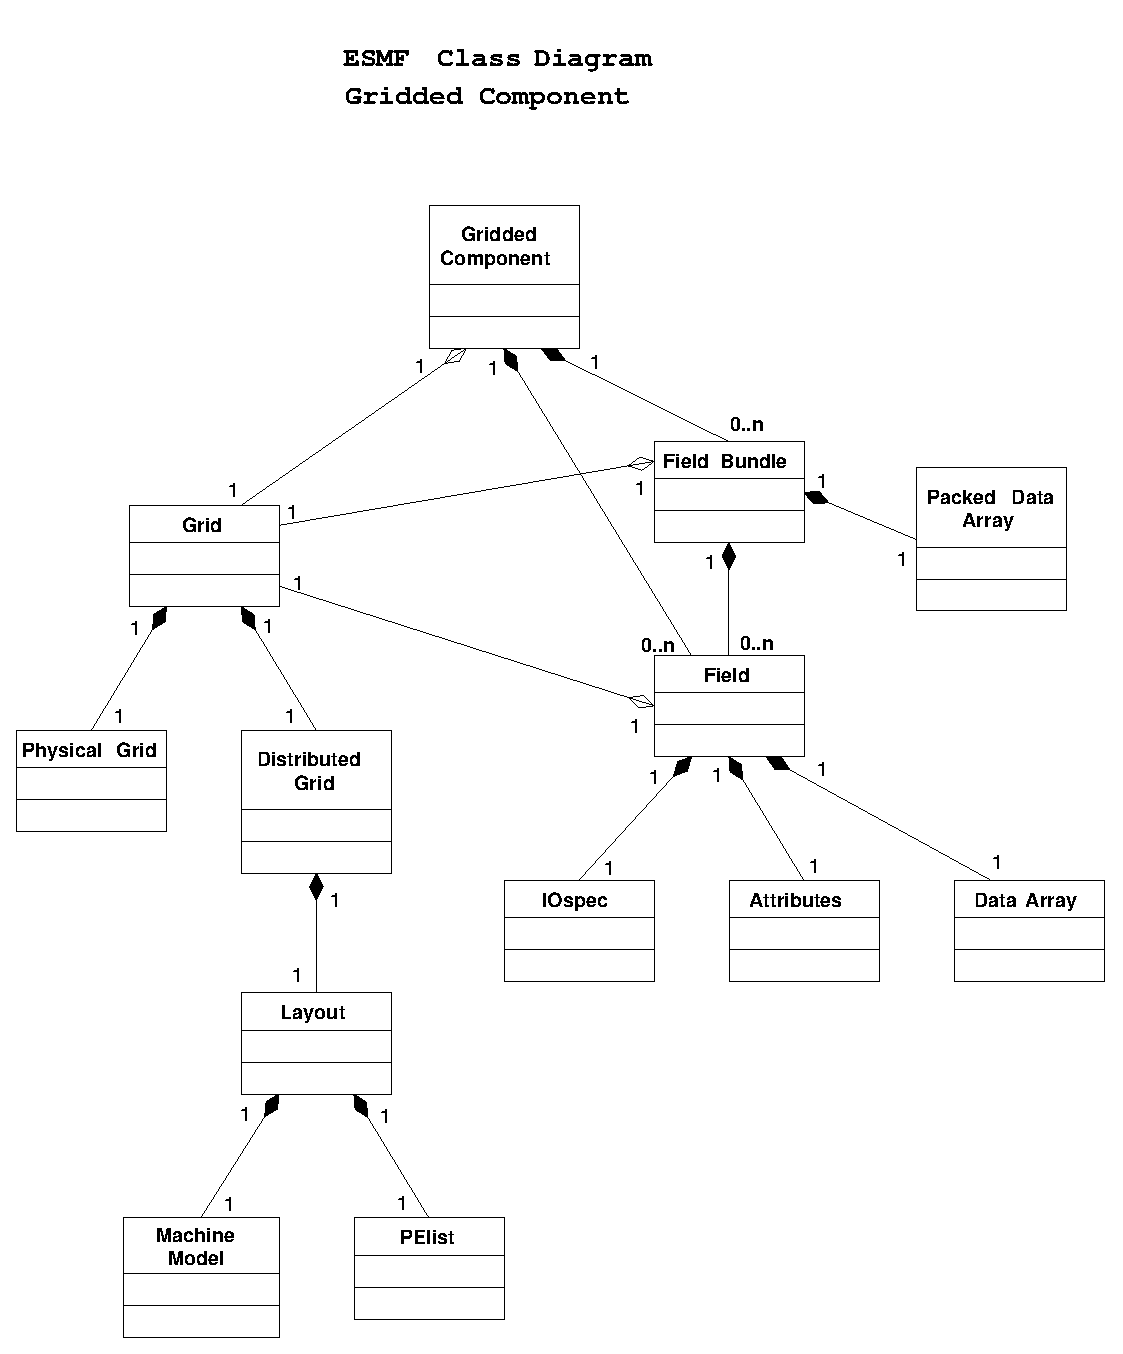
\includegraphics{ESMF_DataStructureHierarchy.eps}}


\subsubsection{Bundle (ESMF\_Bundle)}
\label{sec:bundle} 
\begin{description}
\item [Description] A Bundle contains one or more Fields which are defined on the
same Grid.  It allows the application to manipulate multiple fields in an identical
manner with a single set of calls.  It also allows the option of interleaving data
from multiple fields into a Packed Data Array (see Section~\ref{packeddataarray}) for
more efficient memory access patterns.
\item [Function] The Bundle class is an aggregation of the Field class.  It provides methods 
for getting and setting fields.  It provides methods for querying information about the
underlying grid.  It provides methods for requesting the packing of data, the
reordering of that packed data, and detaching and attaching the data.
\end{description}

\subsubsection{Packed Data Array (ESMF\_PackedData)}
\label{sec:packeddataarray} 
\begin{description}
\item [Description] A Packed Data Array contains data from one or more Fields, where the
data items are interleaved in memory. The application may use a packed array to maintain
locality of reference while iterating the array, or for ease in subsetting multiple
data values in one operation.
\item [Function] The PackedData class provides methods for packing and querying arrays,
subsetting the data, and repacking the data in a different order.  The PackedData object
contains an Ordering object to maintain the information about the structure of the packing.
It is contained by a Bundle object.  Application access is through Bundle methods.
\end{description}

\subsubsection{Field (ESMF\_Field)}
\label{sec:field} 
\begin{description} 
\item [Description] A Field represents a single physical field or the components of a 
vector field.  It is the basic data carrying object in the system.  It includes both
the data and the grid on which the data is defined.  The main application interfaces
for accessing data are here.
\item [Function] The Field object is a composition of the Data Array object, an optional
Mask object, an optional IOspec object, and it aggregates a Grid object.  It provides
methods for getting, setting, and querying the data array, the grid, the mask and
the I/O spec.  It provides methods for detaching and attaching data from the field.
While data is detached it is the responsibility of the application.  A Field object
provides methods for subsetting, regridding, and reordering memory layout of data.
\end{description}

\subsubsection{Mask (ESMF\_Mask)}
\label{sec:mask} 
\begin{description}
\item [Description] A Mask describes a subset of data items, for example to indicate
the valid values which represent ocean points (and not land) in an ocean model.  
It may be specified at the Grid object level, but it is stored below the Field level 
for effiency of computation.
\item [Function] The Mask class is an optional part of a Field class.  It provides methods
for getting and setting valid values.
\end{description}

\subsubsection{Data Array (ESMF\_Data)}
\label{sec:dataarray} 
\begin{description}
\item [Description] A Data Array is a list of data values plus information about
the data itself.
\item [Function] The Data class contains the data as well as information about the data,
including the data type (e.g. float,
integer), the machine type (e.g. IEEE float, Cray float), data count, data dimensionality
(e.g. scalar, vector).  It provides methods for querying all information about the data,
returning a pointer to the memory location of the start of the data, and conversion routines
for altering the characteristics of the data.  Information about how the data array is laid
out in memory is contained in an Ordering class.
\end{description}

\subsubsection{Ordering (ESMF\_Ordering)}
\label{sec:ordering} 
\begin{description}
\item [Description] A Ordering is the description of how multidimentional data have been
linearized in memory.  This includes both multidimensional array index information (e.g. C-order
vs Fortran-order) as well as vector or tensor data item information (e.g. all Xs then all
Ys vs [X,Y], [X,Y] tuples).
\item [Function] An Ordering object is associated with a single Data object.  It provides
methods to query the current memory organization and methods to reorder the Data object.
\end{description}

\subsubsection{Grid (ESMF\_Grid)}
\label{sec:ordering} 
\begin{description}
\item [Description] A Grid is the general representation of the coordinate information for
the computation.  It contains both the logical presenatation of the grid as well as the
decomposition of the grid into subgrids for processing in parallel on a
multiprocessor system.
\item [Function] The Grid class is the composition of a PhysGrid and a DistGrid object.  
It is aggregated into the Field and the Bundle objects.  It provides methods to the
Field and Bundle classes for obtaining coordinate, indexing, and decomposition information.
\end{description}

\subsubsection{Physical Grid (ESMF\_PhysGrid)}
\label{sec:physgrid} 
\begin{description}
\item [Description] A Physical Grid is a discrete representation of a continuous physical space.
There are a multitude of types of physical grids.
The grid contains the physical coordinates, usually indicating where data values are located, but
it could be a parametric description of the actual locations.  
\item [Function] The PhysGrid class maintains a global index space for coordinate information.
It provides methods for creating a variety of grid types, including both reading grid information
and generating grids from parameters.  It provides methods for regridding, or translating
one grid to another, used for example when exchanging data through the coupler between
various components.
The PhysGrid class does not handle grid decomposition issues related to 
distributed processing; see the Distributed Grid object in Section~\ref{distgrid}.
\end{description}

\subsubsection{Distributed Grid (ESMF\_DistGrid)} 
\label{sec:distgrid} 
\begin{description}
\item [Description] A Distributed Grid is a collection of subgrids which
constitute a single logical grid.  The subgrids can be operated on in
parallel on a multiple processor machine.  
\item [Function] The DistGrid class contains the mapping
between the local grid decompositions and the global logical grid. 
It contains methods to 
synchronize data values between the boundaries of subsets, and to
collect and communicate global data values.  It interacts closely with
the Physical Grid object (see Section~\ref{physgrid}).
It uses a Layout object to identify and manage the processing elements 
available for the computation.
\end{description}

\subsubsection{Input/Output Specfication (ESMF\_IOspec)}
\label{sec:iospec} 
\begin{description}
\item [Description] A Input/Output specfication contains all information necessary to
read or write objects.  It includes the destination information (e.g. file), the name,
the format, and any format specific parameters needed to complete the I/O.
\item [Function] The IOspec class is ...   << how does this fit?? >>
\end{description}






\newpage
\begin{htmlonly}
\addcontentsline{toc}{part}{Infrastructure:  Utilities}
\end{htmlonly}
\part{Infrastructure:  Utilities}
\label{part:Infrastructure_Utilities}

%\input{ESMF_utils}
\section{Infrastructure: Utilities}
\label{sec:utilclasses}

\subsection{Introduction}

The previous infrastructure section described the data handling 
objects in ESMF. This section describes the lowest level
objects in the infrastructure layer, the utility classes.
Some of these methods will be called directly by user-supplied
code; others are intended to provide support for internal ESMF 
code.

\subsection{Design Goals and Considerations}

One of the goals of the utility layer is to present a uniform interface
for common system functions.  Hardware platforms often have
different system libraries and methods for accomplishing what are 
logically the same tasks.  Routines in this layer insulate user code 
from these variations so that it is portable from system to system.  

In most cases these utilities occupy the lowest level of the object hierarchy.
Another advantage of isolating them is to help avoid circular referencing.

An important goal of the utility layer is to enhance performance portability and
ease of use by establishing structured machine and programming models.  
The machine model captures the performance critical features of a computing 
platform, encoding information about the hardware configuration in a 
systematic way so that it can be analyzed and manipulated.  The programming
model uses this encoded information to allow the user to create
optimized decompositions using a simple, abstract interface.  More detail
on the progaramming model is presented in Section~\ref{sec:progmodel}.

\subsection{Programming Model}
\label{sec:progmodel}

The ESMF programming model defines abstractions that expose
features of the computing environment to the user.  It must support the 
efficient utilization of system resources such as   
computing hardware, OS, and standard library or vendor-supplied 
software (e.g., MPI or other message-passing software, Posix threads, OMP),
and must present a reasonably simple interface to the application 
developer.  

ESMF abstracts the compute elements over which data and tasks may be
distributed into decomposition elements, or {\tt DE}s, which
are essentially threads.  For MPP architectures in which there
is tyically one thread per process, the {\tt DE} degenerates to a 
process.
Depending on the hardware system, ESMF threads will be to a limited 
extent compatible with user-defined threads.  The user will have 
the option to enable ESMF threading or not.  In the latter case, the
{\tt DE} again degenerates to a process.

{\tt DE}s are organized into topologies, such as a 2D grid, by the 
{\tt Layout} 
class.  A user can create a {\tt Layout} directly, or a {\tt Layout} can be 
constructed automatically in the process of creating a {\tt Distributed 
Grid}.  

The {\tt Layout} for both homogeneous and heterogeneous programming
strategies can be described compactly and precisely by a {\tt Layout 
tuple (Ltuple)} of the form: \\
($D_{1}$, $D_{2}$, ... $D_{n}$), where $D_{n}$ is a representation of
each dimension in the layout.  \\
Each $D_{n}$ takes the form \\
$D_{n}$ = (<$R_{1}$>($N_{1}$,$C_{1}$), <$R_{2}$>($N_{2}$,$C_{2}$), ... <$R_{m}$>$(N_{m}$,$C_{m}$)<$P$>) \\
where \\
$R_{m}$ = number of repetitions \\
$N_{m}$ = number of {\tt DE}s \\
$C_{m}$ = connectivity \\
$P$ = periodic boundary \\

Possible values for connectivity are: \\
0 = remote processes \\
1 = adjacent processes, e.g. processes running on the same node\\
2 = threads with access to the same address space \\
Connectivities may be customized.

Figure \ref{fig:layouts} shows number of examples of {\tt Layout} objects,
together with their {\tt Ltuple} description.

\begin{figure}
\caption[{Sample {\tt Layouts}}]{The {\tt Layout} class offers a way of organizing 
machine information and preferentially distributing data in a systematic
and generic way.}
\label{fig:layouts}
\scalebox{0.7}{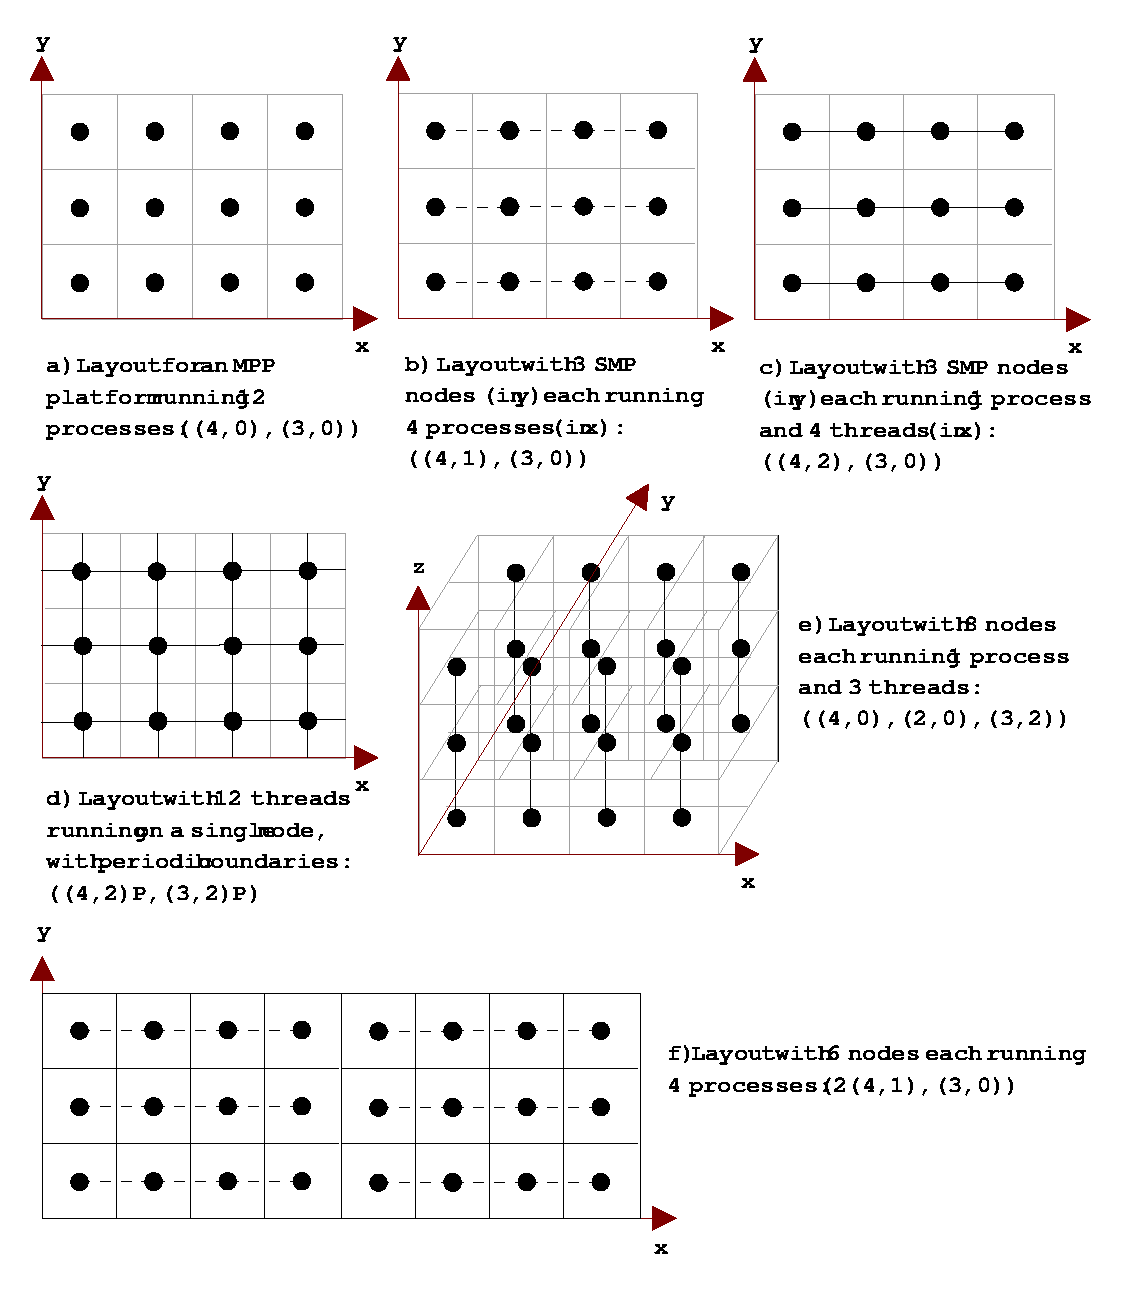
\includegraphics{Layout.eps}}
\end{figure}

When a {\tt Grid} object is defined on a {\tt Layout}, we require that the dimensions 
of the {\tt Grid} align with the dimensions of the {\tt Layout}.  The superimposition
of a {\tt Grid} on a {\tt Layout} is shown in Figure~\ref{fig:gridlayout}.

\begin{figure}
\caption[{{\tt Grid} aligned on a {\tt Layout}}]{The axes of {\tt Grid}s and {\tt Layout}s are aligned.}
\label{fig:gridlayout}
\scalebox{0.7}{\includegraphics{GridLayout.eps}}
\end{figure}

The user can request system resources either through a simple processor
ID list, or by defining a {\tt Layout}.

\subsection{Class Descriptions}

\subsubsection{Base (ESMF\_Base)}
\label{sec:Base} 
All ESMF objects inherit from an ESMF {\tt Base} class.  
The {\tt Base} class is an abstraction of the data and behavior common to all
classes in the framework.  Some methods and data can be
inherited directly; others are expected to be overloaded and/or overridden by
higher level objects.  {\tt Base} class methods include setting and querying 
attributes, print, validate, read/write, and restart. 

\subsubsection{Attributes (ESMF\_Attr)}
\label{sec:Attr}
{\tt Attribute}s are a list of (name, value) pairs associated with any 
object in the library. The value can be of any data type. 
There are methods for listing, setting, and querying attribute lists.
These methods are expected to be implemented in the {\tt Base} class
and not specialized by higher level objects.

\subsubsection{Machine Model (ESMF\_Machine)} 
\label{sec:machine} 
The {\tt Machine Model} provides a general abstraction of 
key, system specific, features of computer hardware and system software in
the ESMF Programming Model.
This information is used by the framework to 
perform resource allocation, data distribution, and dynamic load balancing.  
The {\tt Machine Model} can be queried for information such as
platform type(s), number of processors per node, number of nodes, 
memory attributes and configuration, processor type and speed,
communication semantics and performance, 
interconnect attributes, and system library availability.
It may optionally may provide quantative information 
on actual bandwidth and latency through active tests.  

\subsubsection{PE List (ESMF\_PEList)}
\label{sec:pelist} 
A {\tt PE List} is a list of physical processor IDs.  It includes a 
unique identifier for each {\tt PE} which may differ from the hardware 
processor ID.  

\subsubsection{Layout (ESMF\_Layout)}
\label{sec:layout} 
A {\tt Layout} describes the topology of a set of {\tt Decomposition 
Elements}.
It is used by any part of the ESMF which needs
to decompose a task/problem/dataset into subsets.
The decomposition must allow for mapping certain subsets onto the
underlying machine model in a preferential way; e.g. keeping
vertical blocks of a 3D decomposition on processors which share
a memory pool.  The user may specify generally which 
dimensions of the {\tt Layout} require the most rapid communication.
A user may also explicitly control the {Layout} by specifying which 
communication mechanisms are preferred for a particular dimension.
The {\tt Layout} may interact with both the {\tt PE List}s
and the {\tt Machine Model} in order to accomplish a preferential
decomposition. The layout class will support methods that enable a user or
developer to specify various distributions and fast or slow 
communication axes, e.g. two\_dimensional\_block\_distribute,
cyclic\_distribute, block\_cyclic\_distribute, random\_balanced\_distribute 
etc...


\subsubsection{Basic Communications (ESMF\_Comm)}
\label{sec:basiccomm} 
The {\tt Basic Communication} routines provide a uniform 
interface to the variety of communication mechanisms available
on different hardware platforms.  
The basic functions include methods to send
and receive data, such as scatter, gather, send, receive,
reduction methods such as sum, global min/max, and methods
to synchronize such as barrier. 

\subsubsection{Time Manager (ESMF\_TimeMgr)}
\label{sec:timemgr} 
The {\tt Time Manager} provides general purpose time methods, both
for computing time instants (dates and times) and time intervals
(the difference between 2 time instants).   It also supports 
setting and handling alarm events, either one-shot or repeating.
Supported calendars include Gregorian, Julian, no-leap, 360-day, 
generic, and no-calendar.
Time intervals can range from the very brief -- any rational fraction
of a second -- to geologic time scales.
The {\tt Time Manager} also allows the user to control the format of
time instants and intervals as they are returned.

\subsubsection{Registry (ESMF\_Registry)}
\label{sec:registry} 
A {\tt Registry} maintains a list of (name, ID) pairs per 
namespace.  It supports the many classes in the system which are
required to have unique names, either per address space or over the entire
application.  The {\tt Registry} class provides methods to
create, query, and list namespaces and define their scope.  
Within a namespace it provides methods to
verify a name exists, add a (name, ID) pair,
generate a new unique name, retrieve an ID by name, 
and list existing names.

\subsubsection{Error Handler (ESMF\_Error)}
\label{sec:error} 
The {\tt Error Handler} provides both uniform handling of errors and
a way for users to select how errors will be handled.
An integer error code can be returned from the framework to the
calling code, or the framework can print an error message and exit.
Error messages include information such as the file name, line number, 
and a description of the error.

\subsubsection{Log (ESMF\_Log)}
\label{sec:log} 
The {\tt Log} utility organizes diagnostic output, 
which may be generated in parallel at unpredictable times in
a multiprocessor environment.  It labels the output so that 
searches and filters may be easily constructed.  The quantity of
output is assumed to be moderate to small, i.e. the {\tt Log} 
will not be used to output large streams of numerical model output data.  
It provides methods for writing output and for selecting the
output format, i.e., a single log file vs. a log file per process.

\subsubsection{Diagnostics (ESMF\_Diag)}
\label{sec:diagnostics} 
The {\tt Diagnostic} routines provide assistance with both performance
profiling and code debugging.  Timing routines support measurement
of time intervals at a per-thread granularity around instrumented
sections of code.  Instrumentation links to libraries that can report 
more sophisticated performance statistics if those libraries are available 
on the computing platform.  Debugging routines allow dynamic control over the level
of detail, enabling or disabling of different functional categories,
and assistance with bit-level comparisons for debugging strategies which 
involve running a simulation under differing conditions and
comparing intermediate results.  These routines use methods from
the {\tt Log} class to collect and output results.










\section{Review Status}

\noindent{\bf Architecture Review} \\

\begin{tabular}{r p{1.3in} p{2in}}
{\bf Review Date:} & <Date> \\ \\
{\bf Reviewers:}   & <Reviewer>          & <Institution> \\
                   & <Reviewer>          & <Institution> \\
                   & <Reviewer>          & <Institution>
\end{tabular}

%\section{Glossary}

This glossary defines terms used in Earth system modeling to describe 
parallel computer architectures, grids and grid decompositions, and 
numerical and computational methods.  While some of the concepts in 
the glossary may eventually appear as computational objects, many 
will not.  The goal here is not to define a framework design or an 
object model but simply to achieve a common language.

\begin{description}

\item[Accumulator] \label{glos:Accumulator} A facility for collecting and 
  averaging data values.  Generally accumulators are associated with 
  temporal averaging, although they might be associated with 
  other weighted averaging operations.    
  
\item[Address space] \label{glos:ASP}A standard term to refer to the memory
  seen by a computer program that it can write to directly using
  simple language primitives. 

\item[Alarm] \label{glos:Alarm} An event 
  that occurs at a particular time (or set of times).  It is like an
   alarm on a real alarm clock except that in order to determine whether 
it is "ringing", an alarm is "read" by an explicit application action.

\item[Addressable node] \label{glos:Anode} A set of processors that are
  capable of addressing the same set of blocks of physical memory.

\item[Application] \label{glos:Application} A coherent computational 
  entity run 
  as a single executable or set of communicating executables.  It 
  typically consists of a set of interacting components.

\item[Background grid] \label{glos:BackGrid} 
  A background grid associates each point in a location stream with a 
  location on a grid. A single grid cell may contain zero or more location 
  stream points.  

\item[Bundle] \label{glos:Bundle} A bundle refers to a set of fields that 
  are associated with the same physical grid and distributed in a similar 
  fashion across the same physical axes.  Fields within a bundle may be
  staggered differently and may have different dimensions.

\item[Calendar interval] \label{glos:CalInt} A period of time specified
in calendar-based units that may be used to increment or decrement time instants.  
One year and three months is an example of a calendar interval.  Since 
mathematical operations involving calendar intervals may be ambiguously 
defined -- for example, incrementing January 31 in the Gregorian calendar by 
one month -- default behavior must be carefully specified.  

\item[Cell] \label{glos:Cell} A physical location that is specified by both 
  its extent (vertices) and nominal central location, and is associated with 
  a single integer index value or a set of integer index values ( e.g.
  (i) for 1-d, (i,j) for 2-d, (i,j,k) for 3d ).

\item[Clock] \label{glos:Clock} A clock tracks the passage of time and 
reports the current time instant, like a real clock.  However, most clocks 
used in ESMF components have a key difference to a real clock. Clocks 
in an ESMF component are generally stepped forward by the component, as an 
explicitly coded time step within the overall component.

\item[Component] \label{glos:Component} A large-scale computational entity 
  associated with a particular physical process or computational function, 
  such as a land model.  Components may be generic or user-supplied.  
  See also gridded component, coupler component.

\item[Compute resource] \label{glos:CompResource} Something that appears as a
  physical or virtual computer resource. Example of compute resources
  are a CPU, a network connection, a communication API, a protocol, a 
  particular network fabric or a piece of computer memory. 

\item[Coupler component] \label{glos:Coupler}
  A component that includes all data and actions needed to enable 
  communication between two or more other components.

\item[Data dependency] \label{glos:DataDep} The property of a computational
  operator that defines the data indices required to perform
  the computation at a point.  For instance, a forward differencing
  operation in X at $(i,j)$ has a dependency on $(i+1,j)$.

\item[Data transpose] \label{glos:DataTranspose} Rearrangement of data arrays 
  between two distributed grids sharing the same global domain.

\item[Day of year] \label{glos:DayOfYear} The day number in the calendar year. 
January 1 is day 1 of the year. Day of year expressed in a floating point 
format is used to express the day number plus the time of day. 
For example, assuming a Gregorian calendar:

\begin{tabular}{ll}
{\bf date}              & {\bf day of year} \\
\hline 
10 January 2000, 6Z     & 10.25 \\
31 December 2000, 18Z   & 366.75 
\end{tabular}

\item[DE] \label{glos:DE} 
Short for decomposition element.

\item[Decomposition element (DE)] \label{glos:Decomp_Element}
A decomposition element is a virtual portion of a computer 
associated with a processing element and an address space.  A DE may 
be associated with an MPI process or a thread.  Layouts 
assign a topology to decomposition elements.

\item[Distributed grid] \label{glos:DistGrid}
  A distributed grid defines the decomposition of the global index space 
  across the layout and methods on the indexed data.

\item[Distribution] \label{glos:Distribution} The function that expresses
the relationship between the indices in a distributed grid and the elements 
in a layout.  

\item[Domain decomposition] \label{glos:DomainDecomp} The act of grid 
  distribution: creating a layout; and associating gridpoints with the layout. 
  The dimensionality of the domain decomposition is the dimensionality of 
  the associated layout.

\item [Exact] \label{glos:Exact} The word exact is used
to denote entities, such as time instants and time intervals, for which truncation-free arithmetic is required. 

\item[Exchange grid] \label{glos:ExchangeGrid} A grid whose vertices are
formed by the intersection of the vertices of two overlying grids.  Each 
cell in the exchange grid overlies exactly one cell in each grid of the 
exhange.

\item[Exchange packets] \label{glos:EP} The data exchanged by components.  
  Exchange packets may or may not contain contiguous data, and may contain 
  both field and other forms of data.

\item[Exclusive domain] \label{glos:ExcDomain} The set of indices whose 
  data is exclusively and definitively updated by a particular PE.

\item[Executable] \label{glos:Exec} 
  A parallel program that is under independent control by the operating 
  system.

\item[Export state] \label{glos:ExportState} The data and 
  metadata that a component can make available for exchange 
  with other components. This may be data at a physical boundary 
  (e.g land-atmosphere interface) or in other cases, it might be the 
  entire model state.  See also restart state, import state.

\item[Field] \label{glos:Field} A field is a physical quantity
  defined within a region of space.  A field includes a grid 
  and any metadata necessary for a full description of the field data.

\item[Functionality Class] \label{glos:FuncClass}
A functionality class is a body that accomplishes a given function, such
as I/O. It may contain several different classes or extend over multiple
framework layers. Functionality classes are described in the ESMF Architecture
Document.

\item[Generic component] \label{glos:GenericTrans} A generic component
  is one supplied by the framework.  The user is not expected to 
  customize or otherwise modify it.  See also user component.

\item[Generic transform] \label{glos:GenericTrans} A generic transform 
  is a operation supplied by the framework, for example, a method 
  that converts gridded data from one supported physical grid and/or 
  decomposition to another using a specified technique.  See also user 
  transform.

\item[Global physical grid] \label{glos:GlobPhysGrid} 
  A global physical grid contains physical information about the entire, 
  undecomposed domain.  No distributed grid need be associated with a global 
  physical grid.  

\item[Global domain] \label{glos:GlobDomain}
  The global range of indices of data points.

\item[Global reduction] \label{glos:GlobReduction} 
  Reduction operations (sum, max, min, etc.) on
  data defined on a distributed grid.  See also global broadcast.

\item[Global broadcast] \label{glos:GlobBroadcast}
  Scatter operations on data defined on a distributed grid.
  See also global reduction.

\item[Grid] \label{glos:Grid} The discrete division of space associated with
  a particular coordinate system.  A grid contains all physical grid and memory 
  organization information (via distributed grid and layout) required to manipulate 
  fields, as well as to create and execute grid transforms. 

\item[Grid metrics] \label{glos:GridMetrics} Terms relating measurements 
  in index space to physical grid quantities like distances and areas.

\item[Grid staggering] \label{glos:GridStagger} 
  A descriptor of relative locations
  of scalar and vector data on a structured grid. On different
  staggered grids, vector data may lie at cell faces or vertices,
  while scalar data may lie in the interior. The staggered locations
  are often written in a notation like $(i+\frac12,j+\frac12)$ to
  describe the offset of a corner with respect to the cell $(i,j)$.

\item[Grid topology] \label{glos:GridTopo} Description of data 
  connectivities in index space.

\item[Grid union] \label{glos:GridUnion} The formation of a new grid
  by taking the union of the vertices of two input grids. 

\item[Gridded component] \label{glos:GridComp}
  A component that is associated with one or more grids.  No requirements 
  may be placed on the physical content of a gridded component's data or 
  on the nature of its computations. 

\item[Halo] \label{glos:Halo} 
  The points in the data domain outside the local domain. 

\item[Halo update] \label{glos:HaloUpdate}
  Halo points are associated with other PEs'
  local domains, and the halo update operation involves
  synchronization of some or all halo points with other PEs. 

\item[Import state] \label{glos:ImportState} The data and metadata 
  that a component requires from other components in order to run.  
  See also export state, restart state.

\item[Index] \label{glos:Index} An integer value associated with a set
  of coordinates that describe a cell or location in physical space.

\item[Index space] \label{glos:IndexSpace} The space implied 
  by a set of indices.  An index space has a defined dimensionality and 
  connectivity.

\item[Index space location] \label{glos:IndexSpaceloc} 
  A location within index space.  A index space location may be fractional.
  See also physical location.

\item[Layout] \label{glos:Layout} A layout specifies a PE list, 
  decomposition strategy (thread and process), and the dimensionality 
  and connectivity of the decomposition.  Multiple distributed 
  grids may be defined per layout.

\item[Local domain] \label{glos:LocalDomain} This includes the exclusive 
  domain, as well as the points with whom the exclusive points have data 
  dependencies.

\item[Local physical grid] \label{glos:LocPhysGrid} The portion of a 
  physical grid associated with a local domain.  

\item[Location stream] \label{glos:LocStream} A list of
  locations with no assumed relationship between these locations.  The
  elements of a location stream are assumed to share the same data
  items and metadata, though some elements may have blank entries for
  particular data or attributes.

\item[Logically rectangular grid] \label{glos:RecGrid} A grid in 
  which sequential indices are physically adjacent, and in which the 
  extent of each index is independent of the other indices.

\item[Loose bundle] \label{glos:LooseBundle} A loose bundle consists of 
  fields whose data is not contiguous in memory.

\item[Machine model] A generic representation of the computing 
  platform architecture.

\item[Mask] \label{glos:Mask} A field marking a span within a larger grid.

\item[Memory domain] \label{glos:MemDomain} The portion of memory 
  associated with an local domain.  The memory domain is always at least 
  as large as the local domain.

\item[Memory node] \label{glos:Mnode} A set of processors
  sharing equal flat access to a block of physical memory.

\item[MPMD] \label{glos:MPMD} Multiple Program Multiple Datastream.
  Multiple executables, any of which could itself be an SPMD
  executable, executing independently within an application.

\item [No-leap calendar] \label{glos:NoLeap} Every year uses the same months 
and days per month as in a non-leap year of a Gregorian calendar.

\item[Packed bundle] \label{glos:PackedBundle} A packed bundle is arranged
  so that field data is contiguous in memory.

\item[Partition] \label{glos:Partition} In a multi-threaded application, the subset of a
  computational domain that is associated with a logically independent
  sequence of operations. The logical independence requirement is so
  that partitions may be scheduled as separable concurrent tasks.

\item[PE] \label{glos:PE} Short for processing element.

\item[PE list] \label{glos:PElist} A list of processor IDs associated 
  with a component.  See also layout.

\item[Physical grid] \label{term:PhysGrid} 
  A physical grid contains a variety of information
  on the location in physical space and physical metrics (area,
  grid lengths, etc.) of various grid points.

\item[Physical location] \label{glos:PhysLoc} The point in physical space 
  to which data pertain. 

\item[Platform] \label{glos:Platform} 
  The processor hardware, operating system, compiler and
  parallel library that together form a unique compilation target.

\item[Processing element (PE)] \label{glos:Processing_Element}
A processing element is associated with a single hardware processor.  It may
have a framework ID that is different than its vendor-assigned ID.  

\item[Processing node] \label{glos:Pnode} A set of processors to which an
  operating system scheduler is capable of assigning to a single job.

\item[Restart state] \label{glos:RestartState} The component 
  data that 
  is needed for an exact restart. This can include, in addition to 
  a physical state,  time information, static field data,
  metadata and control information. 

\item[Scheduler] \label{glos:Scheduler} An operating system component 
  that assigns system
  resources (processors, memory, CPU time, I/O channels, etc.) to
  executables.

\item[Span] \label{glos:Span} The physical extent associated with a grid.

\item[SPMD] \label{glos:SPMD} Single Program Multiple Datastream. 
  A single executable, possibly with many 
  components (representing for example the atmosphere, the ocean, 
  land surface) executing serially or concurrently.

\item [System time] \label{SysTime}Time spent doing system tasks such as I/O or in system calls.  May also
include time spent running other processes on a multiprocessor system.

\item [Time instant] \label{glos:TimeInstant}
Generic name for an absolute time and date specification. A time instant is made 
up of a time and date and an associated calendar. It may include a time zone.
``Jan 3rd 1999, 03:30:24.56s, UTC'' is one example of a time instant.

\item [Time interval] \label{glos:TimeInterval} A time interval is the
period between any two time instants, measured in units, such as days, 
seconds, and fractions of a second, that are not associated with a specific
calendar.  Time intervals may be negative.  The periods 2 days and 10 seconds, 
86400 and 1/3 seconds and 31104000.75 seconds are all examples of time intervals.  
Mathematical operations such as addition, multiplication and subdivision 
can be applied to time intervals.

\item [User component] \label{UserComp} A component that is customized or
written by the user.  See also generic component.

\item [User time] \label{UserTime} Processor time actually spent executing a process's code.

\item[User transform] \label{glos:UserTrans} A user-supplied 
  method that is used to extend framework capabilities beyond generic 
  transforms.  

\item [Wall clock time] \label{WallClockTime} Elapsed real-world time (i.e. difference between start time minus
stop time).

\end{description}










































%\section{Bibliography}
%\bibliography{comp} 
%\bibliographystyle{plain}
%\addcontentsline{toc}{section}{Bibliography}

\end{document}







